\documentclass{beamer}

\usecolortheme[RGB={205,173,0}]{structure}

\usepackage[spanish,es-noshorthands]{babel}
\usepackage{tikz}
\usetikzlibrary{calendar}

%\usepackage[spanish,activeacute,es-tabla]{babel}
\usepackage[utf8]{inputenc} % mac utf8
\usepackage{beamerthemesplit}


\usepackage{graphicx}
\DeclareGraphicsExtensions{.png,.pdf,.jpg}

\usefonttheme{professionalfonts} % fuentes de LaTeX 
\usetheme{Dresden}	% tema escogido en este ejemplo 

%\usetheme{Boadilla}
\usepackage{minted}
\usepackage{ucs}



\newtheorem{Teorema}{Teorema} 
\newtheorem{Ejemplo}{Ejemplo} 
\newtheorem{Definicion}{Definici\’on} 
\newtheorem{Corolario}{Corolario} 
\newtheorem{Prueba}{Prueba}
\newtheorem{practica} [Corolario]{Práctica} 
\newtheorem{teorema} [Teorema] {Teorema}
\newtheorem{ejemplo} [Ejemplo] {Ejemplo}
\newtheorem{definicion} [Definicion]{Definición} 
\newtheorem{ejercicio} [Corolario]{Ejercicio} 
\newtheorem{lema} [theorem] {Lema}

\setbeamertemplate{theorems}[numbered] 
\setbeamertemplate{caption}[numbered]


\usebackgroundtemplate{
\includegraphics[width=\paperwidth,height=\paperheight]{./img/logos/back.png}}

\title[]{Tema 3 -  Satisfacción Restricciones}
\author[José A Montenegro (jmmontes@uma.es)]{José A. Montenegro}
\institute{Dpto. Lenguajes y Ciencias de la Computación\\
ETSI Informática. Universidad de Málaga\\
jmmontes@uma.es}
\date{\today}

%\setbeamertemplate{headline}{}


%###########################################################################
% FootLine
%###########################################################################

\setbeamertemplate{footline} {%
\leavevmode%
  \hbox{\begin{beamercolorbox}[wd=.5\paperwidth,ht=2.5ex,dp=1.125ex,leftskip=.3cm plus1fill,rightskip=.3cm]{author in head/foot}%
    \usebeamerfont{author in head/foot}\insertshortauthor 
  \end{beamercolorbox}%
  
  \begin{beamercolorbox}[wd=.5\paperwidth,ht=2.5ex,dp=1.125ex,leftskip=.3cm,rightskip=.3cm plus1fil]{title in head/foot}%
    Sistemas Inteligentes\hfill    \insertpagenumber /\insertdocumentendpage
  \end{beamercolorbox}}%
  \vskip0pt%
}%

%###########################################################################
% Document
%###########################################################################

\begin{document}

%\setbeamertemplate{headline}[title slide]
%\setbeamertemplate{footline}[title slide]


%###########################################################################
% Tíitulo
%###########################################################################
\begin{frame}

\includegraphics[height=0.1\textheight]{./img/logos/logoUma.png} \hspace*{3cm}

\includegraphics[height=0.1\textheight]{./img/logos/logoInf.png}   \hspace*{3.5cm}

\includegraphics[height=0.1\textheight]{./img/logos/logoLcc.png}  

\titlepage


\setbeamertemplate{footline}[body]
\setbeamertemplate{headline}[body]
\end{frame}

%###########################################################################
% Contenidos
%###########################################################################
\small
\section[Resumen]{}
\frame{\tableofcontents}

%%%%%%%%%%%%%%%%%%%%%%%%%%%%%%%%
%%%%%%%%%%%%%%%%%%%%%%%%%%%%%%%%
%SECCION %%%%%%%%%%%%%%%%%%%%%%%%%%%%%%%
%%%%%%%%%%%%%%%%%%%%%%%%%%%%%%%%
%%%%%%%%%%%%%%%%%%%%%% 

%%%%%%%%%%%%%%%%%%%%%%%%%%%%%%%%
%%%%%%%%%%%%%%%%%%%%%%%%%%%%%%%%
%\begin{frame}  \small \begin{ejercicio} \end{ejercicio} \pause \textit{\underline{Solución}}:\\ \end{frame} 
%%%%%%%%%%%%%%%%%%%%%%%%%%%%%%%%
%%%%%%%%%%%%%%%%%%%%%%%%%%%%%%%%
%EJERCICIO %%%%%%%%%%%%%%%%%%%%%%%%%%%%%%%
%%%%%%%%%%%%%%%%%%%%%%%%%%%%%%%%



\section{Introducción}
%%%%%%%%%%%%%%%%%%%%%%%%%%%%%%%%
%%%%%%%%%%%%%%%%%%%%%%%%%%%%%%%%


%%%%%%%%%%%%%%%%%%%%%%%%%%%%%%%%

\begin{frame}  \frametitle{Representaciones factorizadas} \footnotesize

\begin{itemize}
\item En los temas anteriores exploramos problemas que pueden resolverse buscando en un espacio de estados


\item Cada estado era atómico, es decir, era una caja negra sin estructura interna


\item Aquí emplearemos una representación factorizada para cada estado

\begin{itemize}
\item Un conjunto de variables, cada una con su valor
\item Un problema está resuelto cuando cada variable tiene un valor que satisface todas las restricciones sobre dicha variable
\end{itemize}

\end{itemize}

\end{frame} 
%%%%%%%%%%%%%%%%%%%%%%%%%%%%%%%%

\begin{frame}  \frametitle{Representaciones factorizadas} \footnotesize

\begin{itemize}
\item En el tema anterior evaluamos los nodos por una función asociada a cada estado ya que son estados atómicos, F(n).

\item Ahora los estados contienen asignaciones a las variables.	
\end{itemize}

\begin{figure}
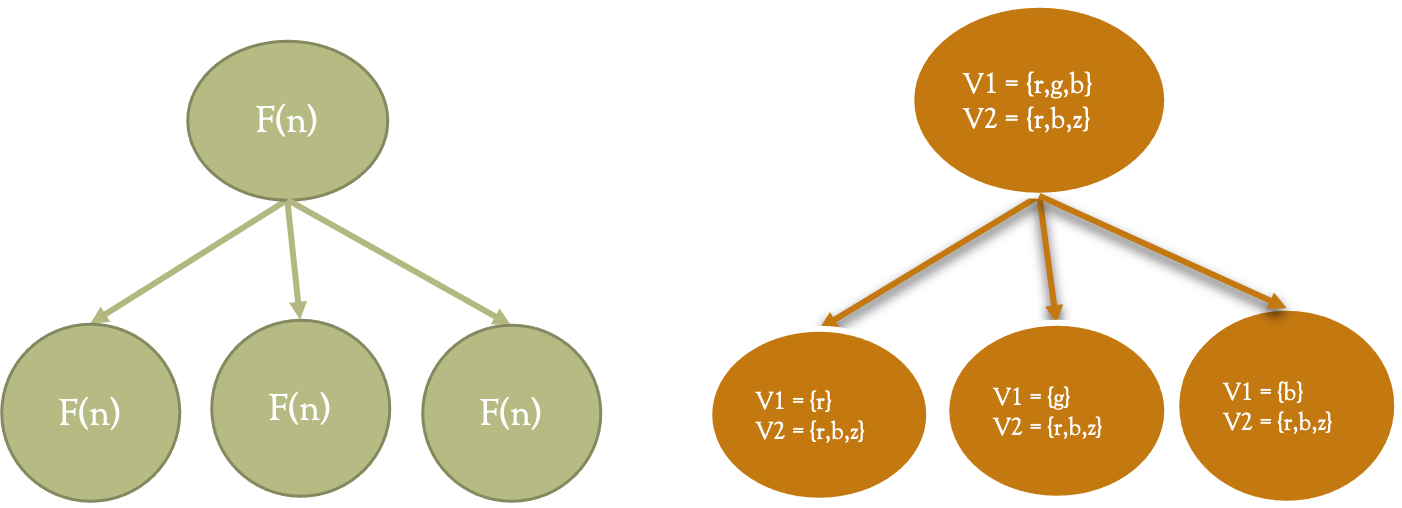
\includegraphics[scale=0.45]{./img/RepresentacionFactorizada}
\end{figure}


\end{frame} 



\section[Definición]{Definición del Problema y Ejemplos}
%%%%%%%%%%%%%%%%%%%%%%%%%%%%%%%%
%%%%%%%%%%%%%%%%%%%%%%%%%%%%%%%%

\begin{frame}  \frametitle{Definición (I)} \footnotesize

\begin{itemize}
\item Un problema de satisfacción de restricciones (constraint satisfaction problem, CSP) está formado por tres componentes:

\begin{itemize}
\item Un conjunto de \textbf{variables}, $X=\{X_1,\ldots ,X_n\}$
\item Un conjunto de \textbf{dominios}, uno para cada variable: $D=\{D1,,\ldots , Dn\}$
\item Un conjunto de \textbf{restricciones} que especifican combinaciones permitidas de valores, C
\end{itemize}

\item Cada dominio $D_i$ es el conjunto de valores posibles$ \{v_1,,\ldots, v_k\}$ para la variable $v_i$.
\end{itemize}

\end{frame} 

%%%%%%%%%%%%%%%%%%%%%%%%%%%%%%%%

\begin{frame}  \frametitle{Definición (II)} \footnotesize

\begin{itemize}
\item Cada restricción $C_i$ es un par $<$scope,rel$>$ donde scope es la tupla de variables que intervienen en la restricción y rel es una relación que define los valores que dichas variables pueden tomar.

\begin{itemize}
\item Por ejemplo, si las variables $X_3$ y $X_5$ deben tener valores distintos, podemos escribir esta restricción como $< (X_3,X_5), X_3 \neq X_5 >$

\end{itemize}

\end{itemize}

\end{frame} 

%%%%%%%%%%%%%%%%%%%%%%%%%%%%%%%%

\begin{frame}  \frametitle{Definición (III)} \footnotesize

\begin{itemize}
\item Cada \textbf{estado} de un CSP se define como una asignación de valores a algunas o a todas las variables,$ {X_i=v_i, X_j=v_j,\ldots }$

\item Una asignación que no viola ninguna restricción se llama \textbf{asignación consistente} o legal


\item Si tenemos una asignación en la cual todas las variables están asignadas, la llamamos \textbf{asignación completa}. 
\begin{itemize}
\item En otro caso, la llamamos \textbf{asignación parcial}.
\end{itemize}

\item Una \textbf{solución} de un CSP es una asignación consistente y completa



\end{itemize}

\end{frame} 

%%%%%%%%%%%%%%%%%%%%%%%%%%%%%%%%

\begin{frame}  \frametitle{Ejemplo 1: Coloreado de mapas} \footnotesize

\begin{itemize}



\item La tarea consiste en colorear cada región de un mapa de tal manera que no haya regiones adyacentes que tengan el mismo color
\item Para el mapa de Australia (siguiente transparencia), definimos las variables como X=\{WA, NT, Q, NSW, V, SA, T\}
\item El dominio de cada variable es $D_i=\{red, green, blue\}$
\item Hay nueve restricciones: C=$\{SA \neq WA, SA \neq NT, SA\neq Q, SA \neq NSW, SA \neq V , SA\neq V, WA\neq NT , NT \neq Q, Q \neq NSW, NSW \neq V\}$


\end{itemize}

\end{frame} 

%%%%%%%%%%%%%%%%%%%%%%%%%%%%%%%%

\begin{frame}  \frametitle{Ejemplo 1: Coloreado de mapas} \footnotesize

\begin{figure}
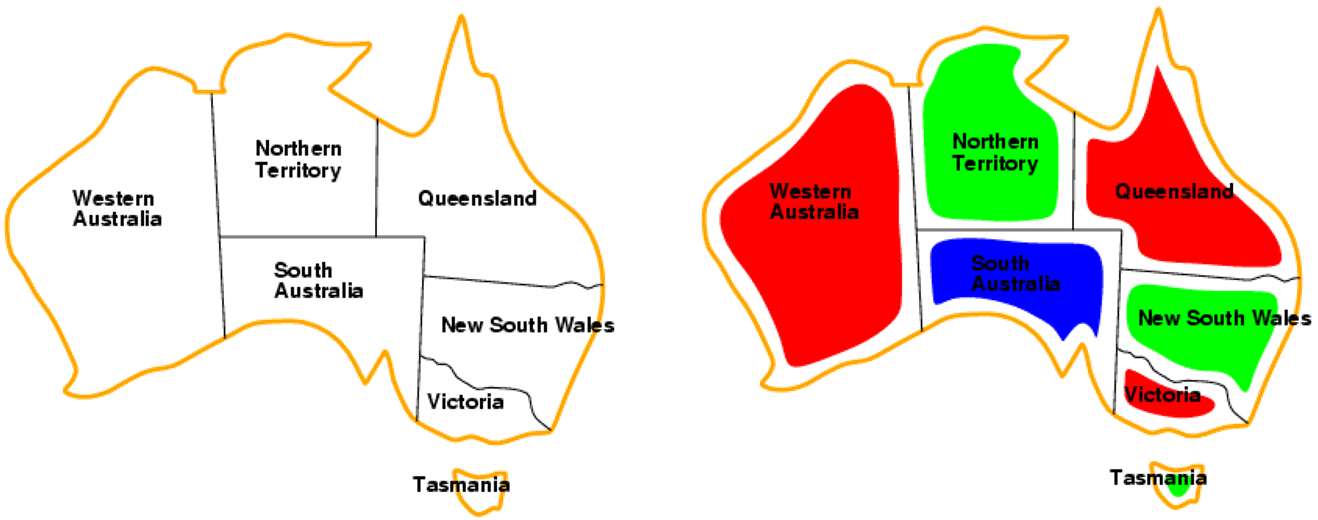
\includegraphics[scale=0.45]{./img/MapaAustralia}
\end{figure}

\begin{itemize}
\item Ejemplo de solución completa y consistente:\\
 WA = red, NT = green, Q = red, NSW = green, V = red, SA = blue, T = green

\end{itemize}

\end{frame} 


%%%%%%%%%%%%%%%%%%%%%%%%%%%%%%%%

\begin{frame}  \frametitle{Ejemplo 1: Coloreado de mapas} \footnotesize

\begin{figure}
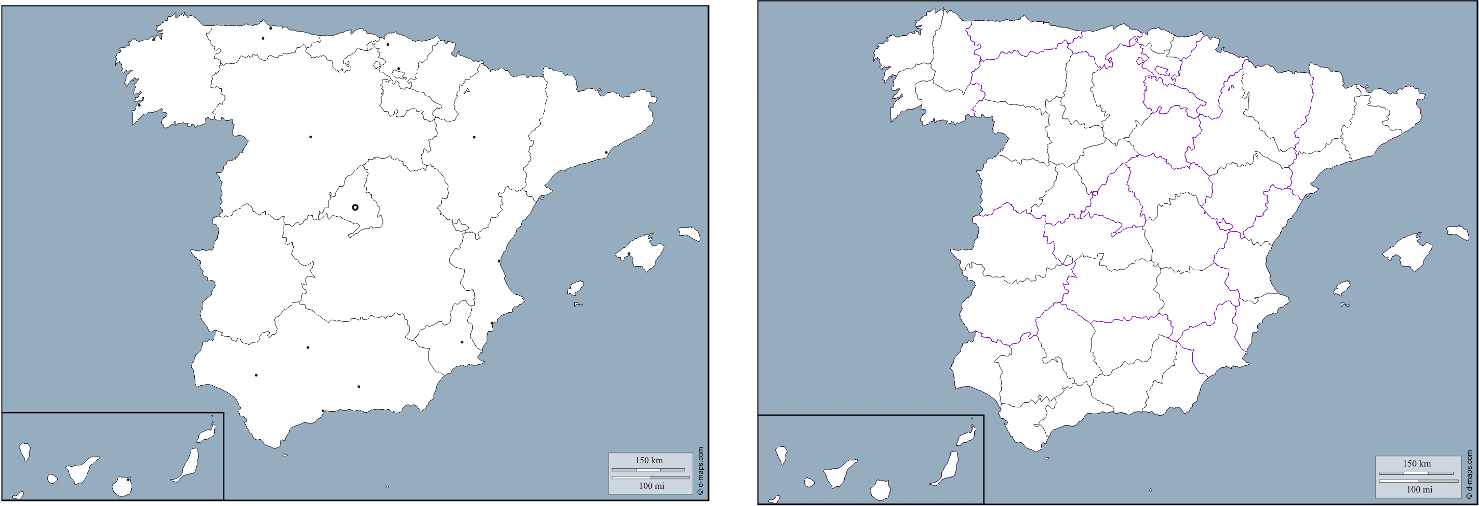
\includegraphics[scale=0.45]{./img/MapaEspaña}
\end{figure}


\end{frame} 

%%%%%%%%%%%%%%%%%%%%%%%%%%%%%%%%

\begin{frame}  \frametitle{Ejemplo 2: problemas criptoaritméticos} \footnotesize

En un acertijo criptoaritmético, cada letra representa a un dígito distinto (0-9)

\begin{figure}

\includegraphics[scale=0.45]{./img/Cripto}
\end{figure}


\end{frame} 

%%%%%%%%%%%%%%%%%%%%%%%%%%%%%%%%

\begin{frame}  \frametitle{Ejemplo 2: problemas criptoaritméticos} \footnotesize

\begin{itemize}
\item El requisito de que todas las variables han de tomar diferentes valores se corresponde con la restricción $AllDiff(F,T,U,W,R,O)$
\item Introducimos tres variables auxiliares $C_{10}, C_{100} y C_{1000}$, que representan los dígitos acarreados a las columnas de las decenas, las centenas y los millares, respectivamente.

\item De esta manera el resto de las restricciones son:

\begin{itemize}
\item $O+O          = R+10 * C_{10}$
\item  $C_{10}+W+W  = U+10 * C_{100}$
\item $C_{100}+T+T   = O+10 * C_{1000}$
\item $C_{1000}               = F$
\end{itemize}

\end{itemize}


\end{frame} 


%%%%%%%%%%%%%%%%%%%%%%%%%%%%%%%%

\begin{frame}  \frametitle{Ejemplo 2: problemas criptoaritméticos} \footnotesize
Solución del acertijo criptoaritmético

\begin{itemize}
\item Variables: $  T, W, 0,U, F, R,C_1,C_2,C_3$
\item Dominios:  \\$T = W= 0 = U = F = R = \{0,1,2,3,4,5,6,7,8,9\}	$\\	$C_1,C_2,C_3 = $ \{0,1\}
 
\item Restricciones:\\ 
$AllDiff(F,T,U,W,R,O)$\\
R + $C_1$ *10    =  0 + 0     	 \\
U + $C_2$ *10    =  W +W + $C_1$\\
O + $C_3$ *10    =  T + T + $C_2$\\
F                      = $C_3$\\
\end{itemize}


\begin{figure}

\includegraphics[scale=0.25]{./img/Cripto}
\end{figure}

\end{frame} 

%%%%%%%%%%%%%%%%%%%%%%%%%%%%%%%%

\begin{frame}  \frametitle{Ejemplo 3: N-Reinas} \footnotesize

\begin{center}
Una variable por cada casilla
\end{center}

\begin{itemize}
\item Variables: $  X_{ij}$
\item Dominios:  $ \{0,1\}	$
\item Restricciones:\\ 

\begin{itemize}
\item  $ {\scriptstyle \forall i,j,k (X_{ij}, X_{ik})   \in   \{(0,0),(0,1),(1,0)\}            \rightarrow  X_{ij} + X_{ik} \leq 1 }$ (h)

\item  ${\scriptstyle \forall i,j,k (X_{ij}, X_{kj})   \in   \{(0,0),(0,1),(1,0)\}            \rightarrow  X_{ij} + X_{kj} \leq 1}$ (v)

\item  ${\scriptstyle \forall i,j,k (X_{ij}, X_{(i+k)(j+k)})   \in   \{(0,0),(0,1),(1,0)\}            \rightarrow  X_{ij} + X_{(i+k)(j+k)} \leq 1}$   (d1)

\item  ${\scriptstyle \forall i,j,k (X_{ij}, X_{(i+k)(j-k)})   \in   \{(0,0),(0,1),(1,0)\}            \rightarrow  X_{ij} + X_{(i+k)(j-k)} \leq 1}$ (d2)

\item ${\scriptstyle \sum_{i,j} X_{ij} = N}$
 
\end{itemize}
\end{itemize}


\begin{figure}
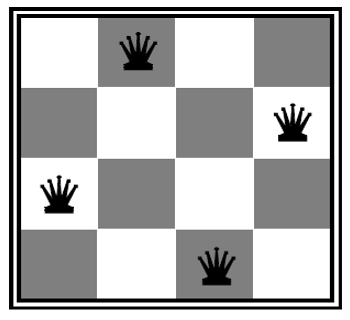
\includegraphics[scale=0.4]{./img/Nreinas}
\end{figure}

\end{frame} 

%%%%%%%%%%%%%%%%%%%%%%%%%%%%%%%%

\begin{frame}  \frametitle{Ejemplo 3: N-Reinas} \footnotesize

\begin{center}
Una variable por cada fila
\end{center}

\begin{itemize}
\item Variables: $  Q_{i}$
\item Dominios:  $ \{1,2,3,\ldots, N	\}	$
\item Restricciones:\\ 

\begin{itemize}
\item Implícito   $  \forall i,j$ no ataca $(Q_i,Q_j)$
\item Explícito  Por ejemplo: $  (Q_1,Q_2) \in \{(1,3),(1,4),\ldots \} $

\end{itemize}


\end{itemize}
\begin{figure}

\includegraphics[scale=0.4]{./img/Nreinas2}
\end{figure}

\end{frame} 


\section[Restricciones]{Restricciones y Consistencia}
%%%%%%%%%%%%%%%%%%%%%%%%%%%%%%%%
%%%%%%%%%%%%%%%%%%%%%%%%%%%%%%%%

%%%%%%%%%%%%%%%%%%%%%%%%%%%%%%%%

\begin{frame}  \frametitle{Tipos de restricciones} \small



\begin{itemize}
\item Una  \textbf{restricción unaria} restringe el valor de una sola variable.

Por ejemplo, para imponer que South Australia no se coloree de verde escribimos $<(SA),SA \neq green>$

\item Una r\textbf{estricción binaria} relaciona dos variables.

Por ejemplo,  $SA \neq  NSW$

\item Una restricción en la que participa un número arbitrario de variables se llama \textbf{restricción global}.\\

Por ejemplo,  $AllDiff(F,T,U,W,R,O)$


\end{itemize}


\end{frame} 

%%%%%%%%%%%%%%%%%%%%%%%%%%%%%%%%

\begin{frame}  \frametitle{Grafo de restricciones} \small


Cada variable se representa mediante un nodo, y cada restricción binaria se representa con un arco

\begin{figure}
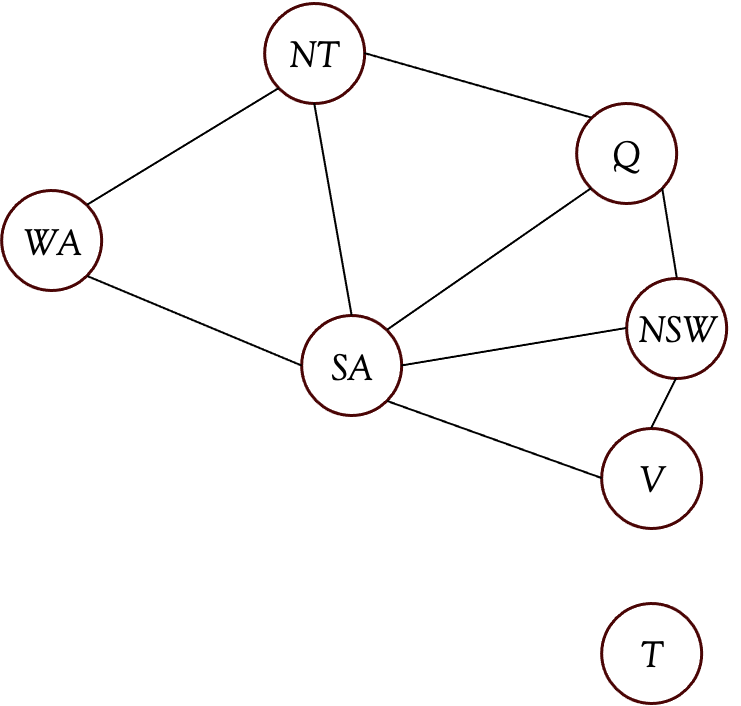
\includegraphics[scale=0.4]{./img/Grafo}
\end{figure}

\end{frame} 

%%%%%%%%%%%%%%%%%%%%%%%%%%%%%%%%

\begin{frame}  \frametitle{Hipergrafo de restricciones} \small


Los recuadros representan las restricciones globales

\begin{figure}
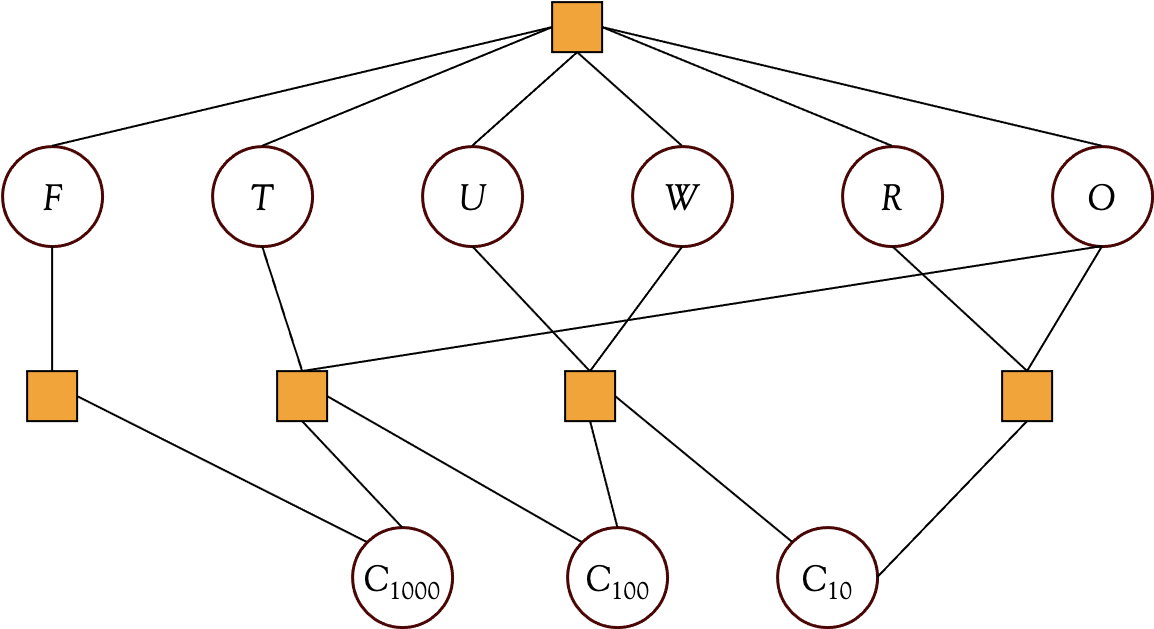
\includegraphics[scale=0.4]{./img/HiperGrafo}
\end{figure}

\end{frame} 

\section[Propagación]{Propagación de Restricciones}
%%%%%%%%%%%%%%%%%%%%%%%%%%%%%%%%
%%%%%%%%%%%%%%%%%%%%%%%%%%%%%%%%

%%%%%%%%%%%%%%%%%%%%%%%%%%%%%%%%

\begin{frame}  \frametitle{Inferencia en CSPs} \small

\begin{itemize}
\item Los problemas de búsqueda en el espacio de estados, solamente podemos buscar.
\item CSPs tenemos dos posibilidades:
\begin{enumerate}
\item Podemos realizar una búsqueda, escoger una asignación entre varias posibilidades.
\item Realizar una tipo de inferencia, denominada propagación de restricciones, utilizando las restricciones para reducir el número de valores legales.
\end{enumerate}

\end{itemize}

\end{frame} 

%%%%%%%%%%%%%%%%%%%%%%%%%%%%%%%%

\begin{frame}  \frametitle{Inferencia en CSPs} \small

\begin{itemize}
\item La propagación de restricciones se pueden intercalar con la búsqueda o como paso previo a la búsqueda.

\item Dependiendo del problema con la propagación de restricciones es suficiente para encontrar una solución y no es necesario realizar la búsqueda.
\item La idea es mantener la consistencia en el grafo de restricciones.

\end{itemize}

\end{frame} 

%%%%%%%%%%%%%%%%%%%%%%%%%%%%%%%%

\begin{frame}  \frametitle{Consistencia de nodos} \small

\begin{itemize}
\item Una variable es \textbf{nodo-consistente} si todos los valores del dominio de la variable satisfacen las \textbf{restricciones unarias} sobre dicha variable.

Por ejemplo, si tenemos la restricción unaria $<(SA),SA \neq green>$, podemos hacer SA nodo-consistente quitando green de su dominio, lo que deja a SA con el dominio reducido {red, blue}

\item Siempre es posible eliminar todas las restricciones unarias de un CSP ejecutando la consistencia de nodos.

\end{itemize}

\end{frame} 

%%%%%%%%%%%%%%%%%%%%%%%%%%%%%%%%

\begin{frame}  \frametitle{Consistencia de arcos} \small

\begin{itemize}
\item Una variable $X_i$ es arco-consistente si, para cada valor del dominio de $X_i$ y cada \textbf{restricción binaria} $(X_i,X_j)$, podemos encontrar al menos un valor en el dominio de $X_j$ que satisface la restricción

\item Una red es arco-consistente si toda variable es arco-consistente con las demás variables

\item El siguiente algoritmo asegura la arco-consistencia de la variable $X_i$ con respecto a otra variable $X_j$; devuelve true si y sólo si se ha revisado el dominio de $X_i$.

\end{itemize}

\end{frame} 

%%%%%%%%%%%%%%%%%%%%%%%%%%%%%%%%
\subsection{Algoritmo de revisión de dominios}
%%%%%%%%%%%%%%%%%%%%%%%%%%%%%%%%

%%%%%%%%%%%%%%%%%%%%%%%%%%%%%%%%

\begin{frame}  \frametitle{Algoritmo de revisión de dominios} \footnotesize


\begin{figure}
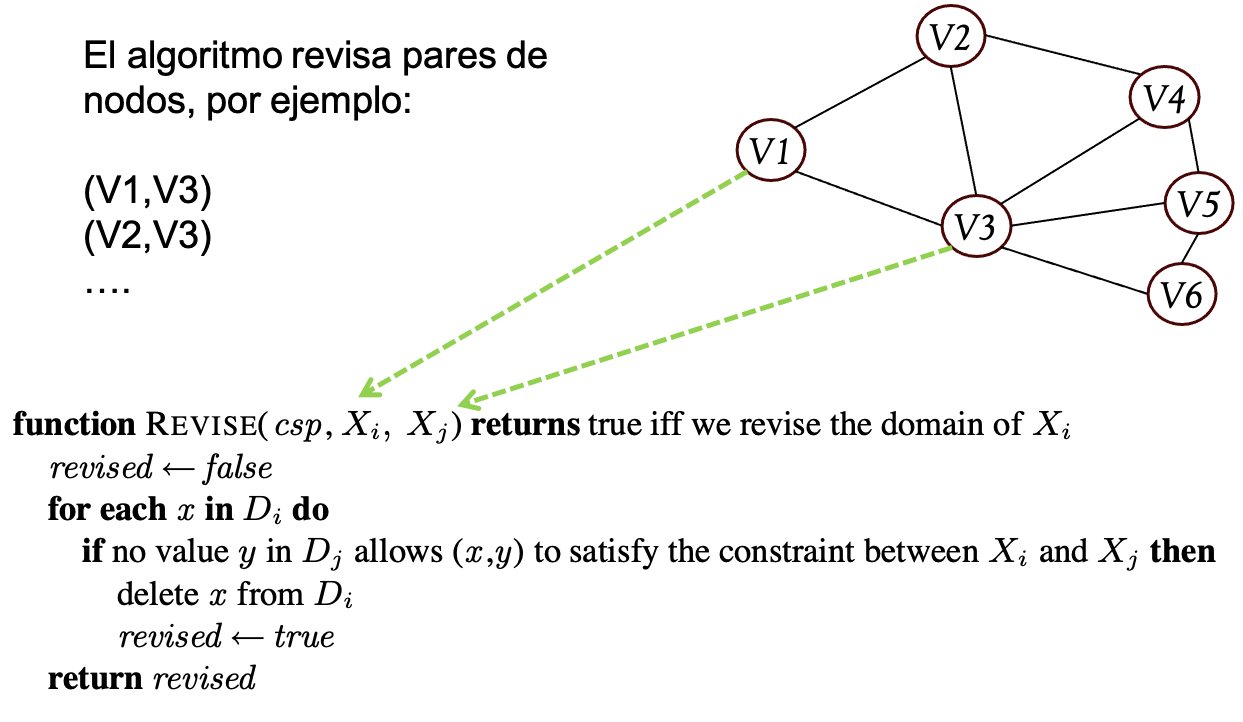
\includegraphics[scale=0.5]{./img/RevisionDominios}
\end{figure}
\end{frame} 

%%%%%%%%%%%%%%%%%%%%%%%%%%%%%%%%

\begin{frame}  \frametitle{Algoritmo de revisión de dominios} \footnotesize

\begin{tabular}{ll}
\textbf{Ejemplo}:					& 	Revised = false\\

$X_i = V_1 X_j = V_2$		&  $D_i = \{g,b\} D_j = \{r\}$\\

$V_1= \{g,b\} V_2 = \{r\}$ 	&  1.(g,r) Satisface las Restricciones\\

$V_1 \neq V_2$  				& 2.(b,r) Satisface las Restricciones\\
										& RETURN false  \\
\end{tabular} 


\begin{figure}

\includegraphics[scale=0.5]{./img/Revise}
\end{figure}



\end{frame} 


%%%%%%%%%%%%%%%%%%%%%%%%%%%%%%%%

\begin{frame}  \frametitle{Algoritmo de revisión de dominios} \footnotesize

\begin{tabular}{ll}
\textbf{Ejemplo}:					& 	Revised = false \\

$X_i = V_1 X_j = V_2$		&  $D_i = \{g,b\} D_j = \{b\}$  \\

$V_1= \{g,b\} V_2 = \{b\}$ 	&  1.(g,b) Satisface las Restricciones  \\

$V_1 \neq V_2$  				& 2.(b,b)  \textbf{NO} Satisface las Restricciones \\
										& 	 \hspace{1mm} a. Modifico $D_i,  D_i = \{g,b\}  D_i = \{g\}$\\
\textbf{Salida}: 					& 	 \hspace{1mm} b. Revised = true\\
$V_1= \{g\} V_2 = \{b\}$   	&   RETURN false  \\
\end{tabular} 


\begin{figure}

\includegraphics[scale=0.5]{./img/Revise}
\end{figure}


\end{frame} 


%%%%%%%%%%%%%%%%%%%%%%%%%%%%%%%%
\subsection{Algoritmo AC-3}
%%%%%%%%%%%%%%%%%%%%%%%%%%%%%%%%

%%%%%%%%%%%%%%%%%%%%%%%%%%%%%%%%

\begin{frame}  \frametitle{Algoritmo AC-3 } \small

\begin{itemize}
\item El algoritmo más popular para asegurar la arco-consistencia en una red se llama AC-3
\item Inicialmente el conjunto contiene todos los arcos del CSP
\item A continuación extrae un arco cualquiera $(X_i,X_j)$ del conjunto y hace $X_i$ arco-consistente con respecto a $X_j$ 

 Si esto reduce el dominio $D_i$, entonces añadimos al conjunto todos los arcos $(X_k,X_i)$, tales que $X_k$ es vecino de $X_i$

\item Si un dominio se reduce a nada, entonces el CSP original no tenía solución, y devolvemos false. 

En otro caso obtenemos un CSP en el que es más fácil buscar.

\end{itemize}

\end{frame} 
%%%%%%%%%%%%%%%%%%%%%%%%%%%%%%%%

\begin{frame}  \frametitle{Algoritmo AC-3 } \small

\begin{figure}
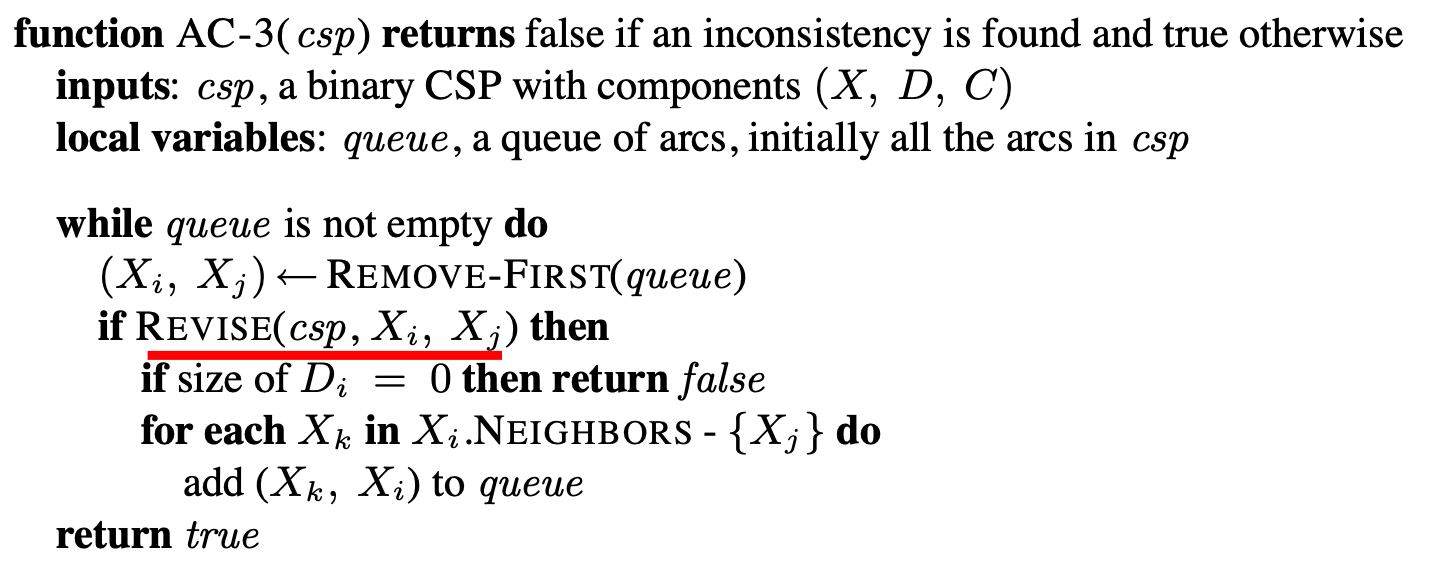
\includegraphics[scale=0.45]{./img/Ac3}
\end{figure}

\end{frame} 

%%%%%%%%%%%%%%%%%%%%%%%%%%%%%%%%

\begin{frame}  \frametitle{Ejemplo Algoritmo AC-3 } \small

Consideramos el siguiente problema:

\begin{itemize}
\item Tres variables:  $V_1, V_2, V_3$
\item  Los dominios son: $D_1 = \{b\}, D_2 = \{r,g\}, D_3 = \{g,b\}$
\item Las restricciones son: $V_1 \neq V_2, V_1 \neq V_3,  V_2 \neq V_3$
\end{itemize}
	
Construimos el grafo de restricciones:
	
\begin{figure}
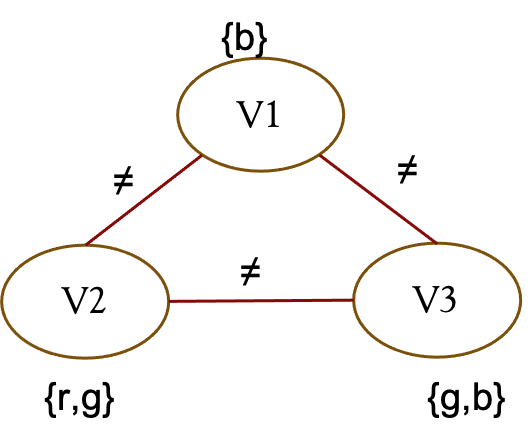
\includegraphics[scale=0.4]{./img/GrafoAC3}
\end{figure}

\end{frame} 


%%%%%%%%%%%%%%%%%%%%%%%%%%%%%%%%

\begin{frame}  \frametitle{Ejemplo Algoritmo AC-3 } \small

\begin{figure}
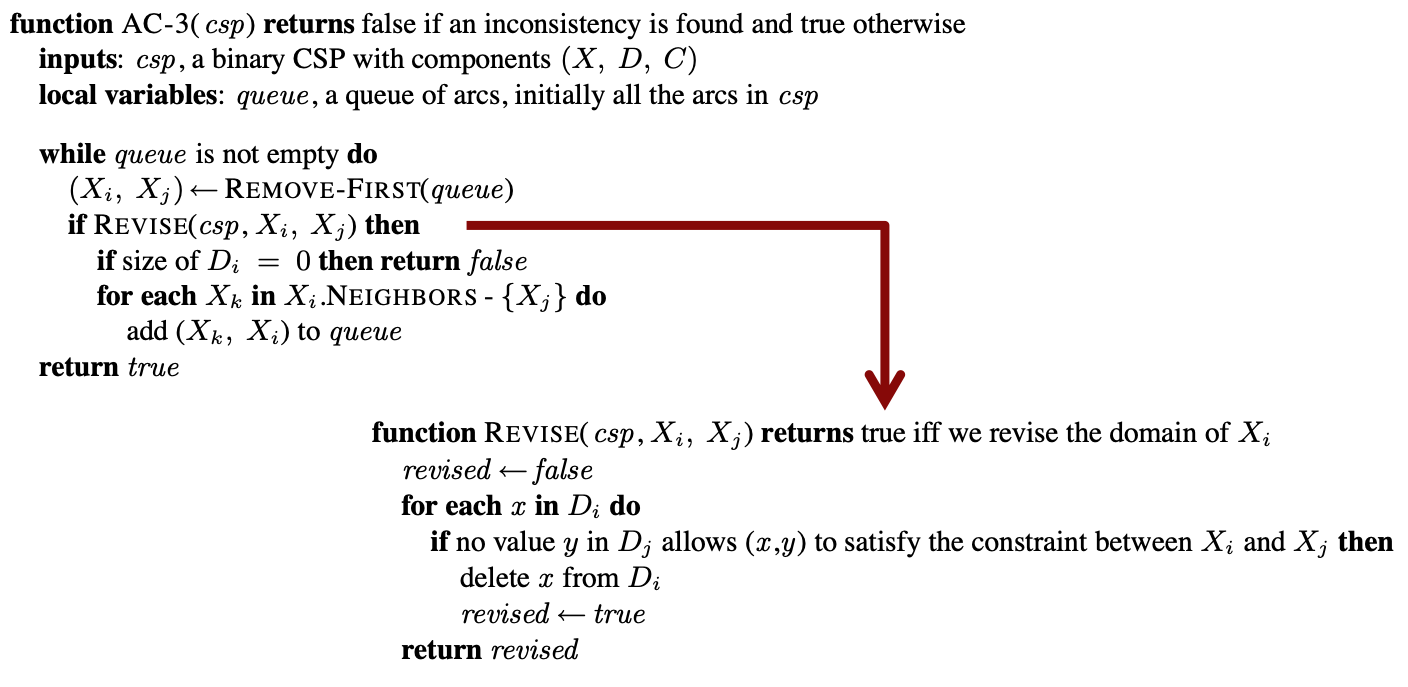
\includegraphics[scale=0.45]{./img/EjAC3}
\end{figure}

\end{frame} 

%%%%%%%%%%%%%%%%%%%%%%%%%%%%%%%%

\begin{frame}  \frametitle{Ejemplo Algoritmo AC-3 } \small

\begin{figure}
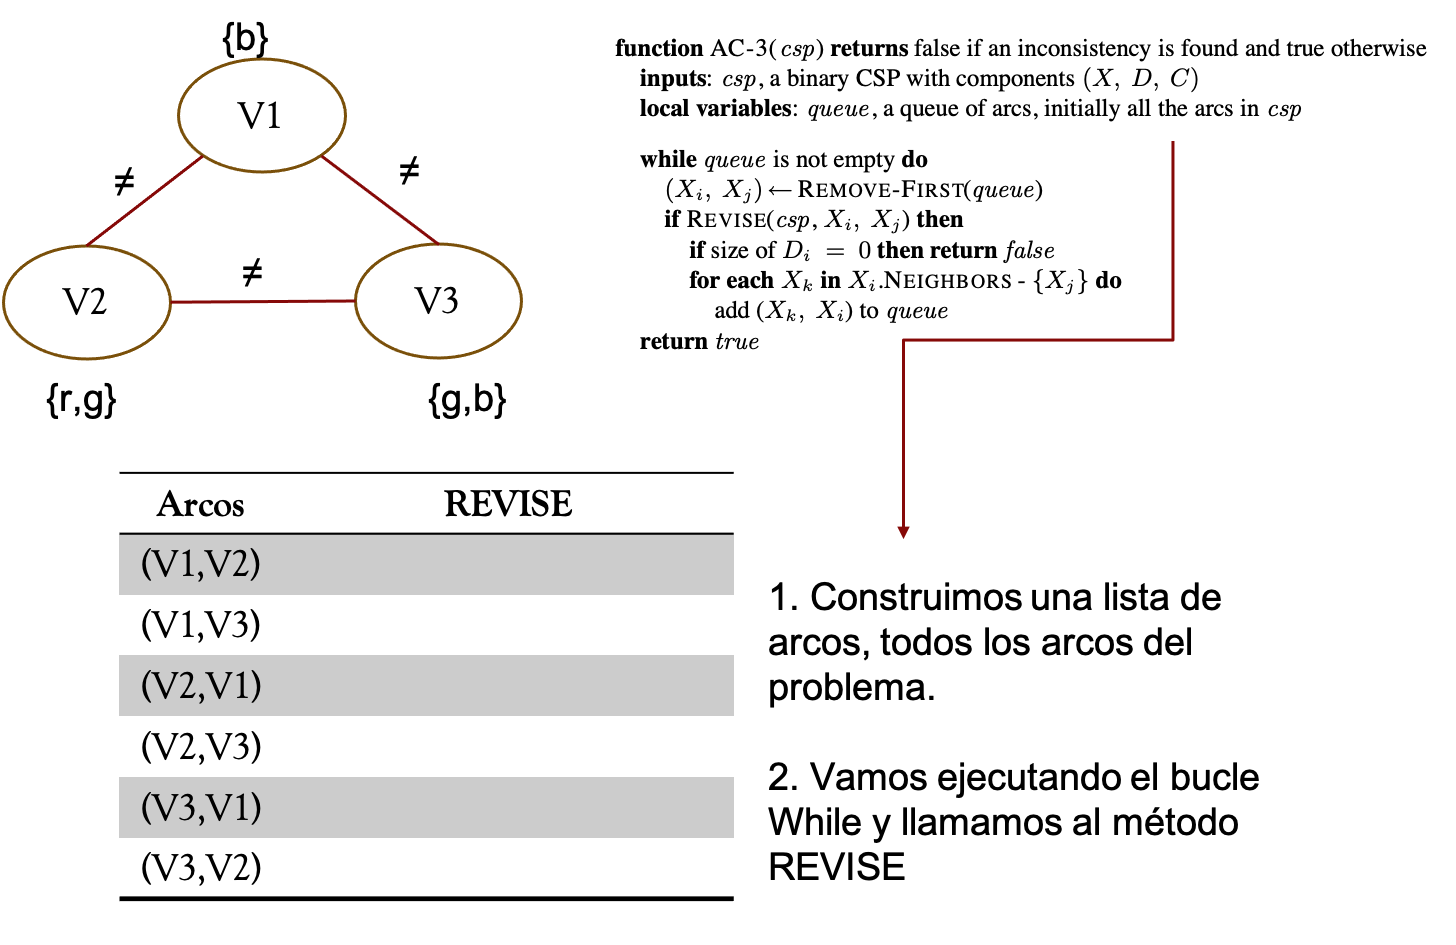
\includegraphics[scale=0.4]{./img/EjAC3_1}
\end{figure}

\end{frame} 

%%%%%%%%%%%%%%%%%%%%%%%%%%%%%%%%

\begin{frame}  \frametitle{Ejemplo Algoritmo AC-3 } \small

\begin{figure}
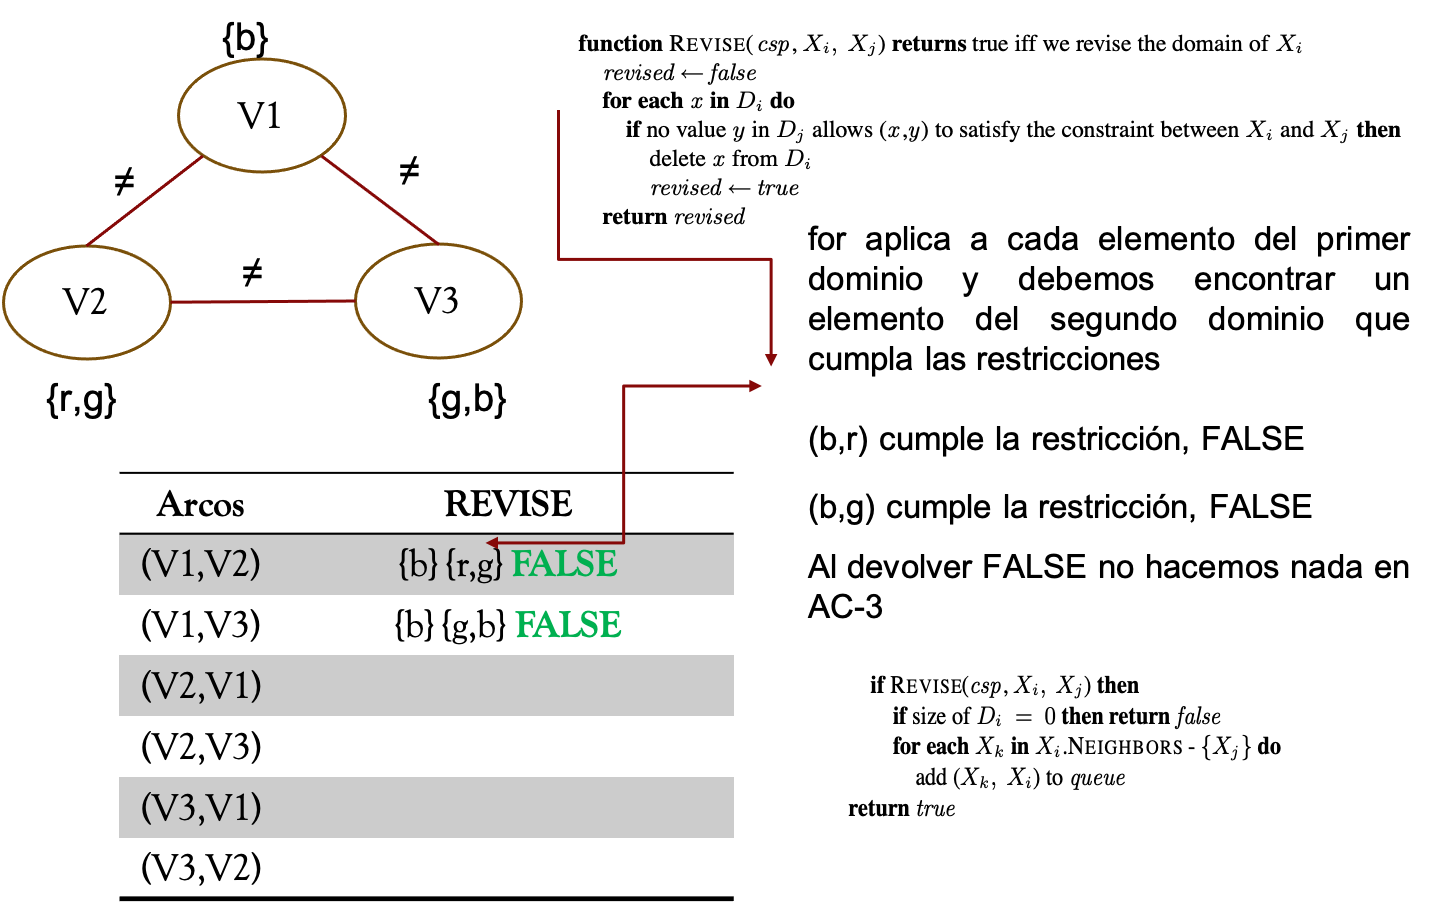
\includegraphics[scale=0.4]{./img/EjAC3_2}
\end{figure}

\end{frame} 

%%%%%%%%%%%%%%%%%%%%%%%%%%%%%%%%

\begin{frame}  \frametitle{Ejemplo Algoritmo AC-3 } \small

\begin{figure}
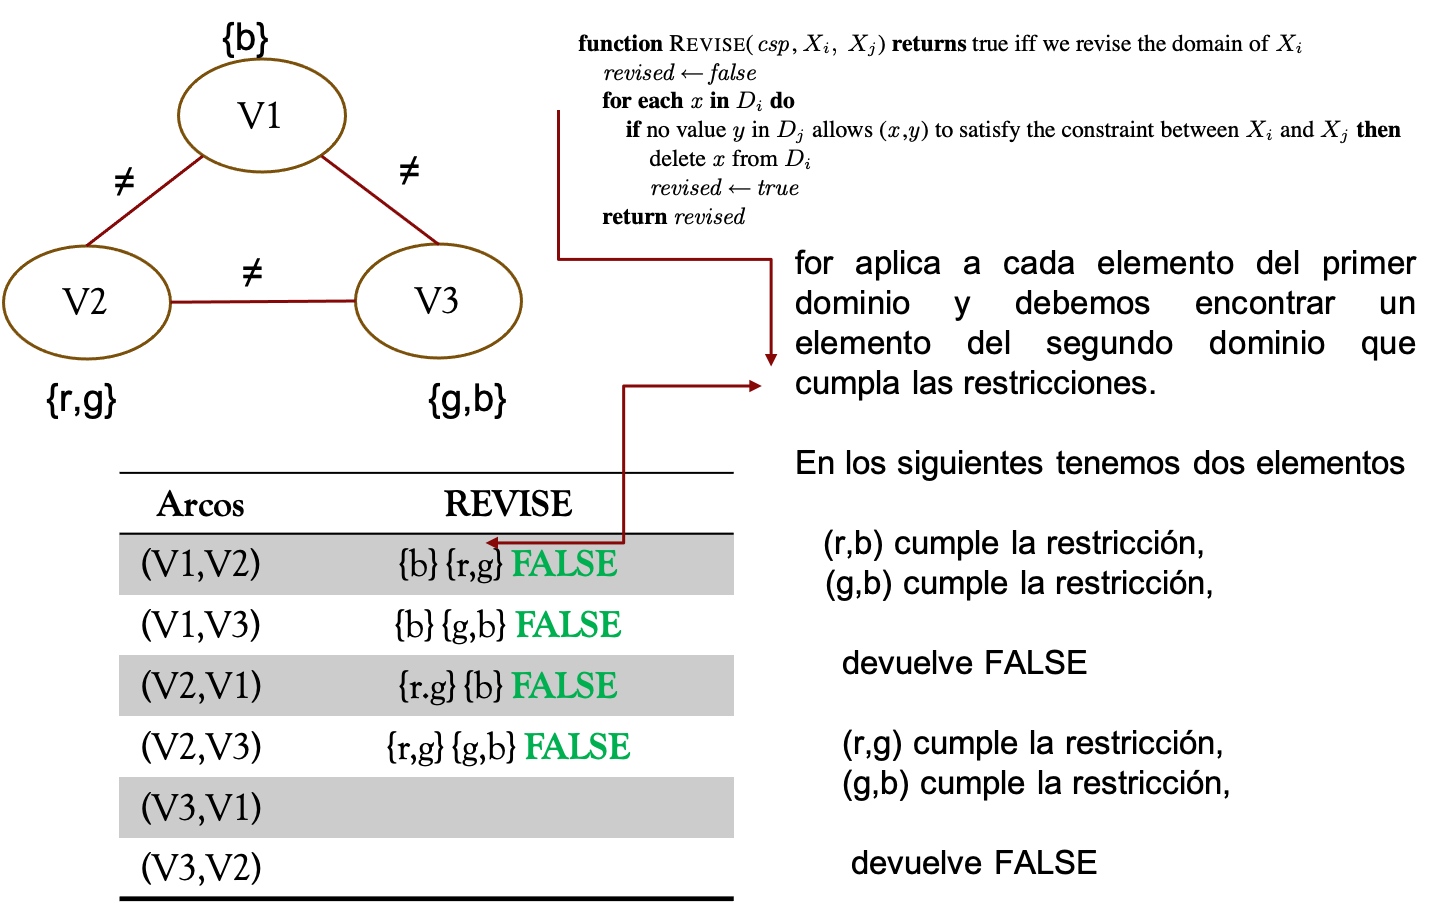
\includegraphics[scale=0.4]{./img/EjAC3_3}
\end{figure}

\end{frame} 


%%%%%%%%%%%%%%%%%%%%%%%%%%%%%%%%

\begin{frame}  \frametitle{Ejemplo Algoritmo AC-3 } \small

\begin{figure}
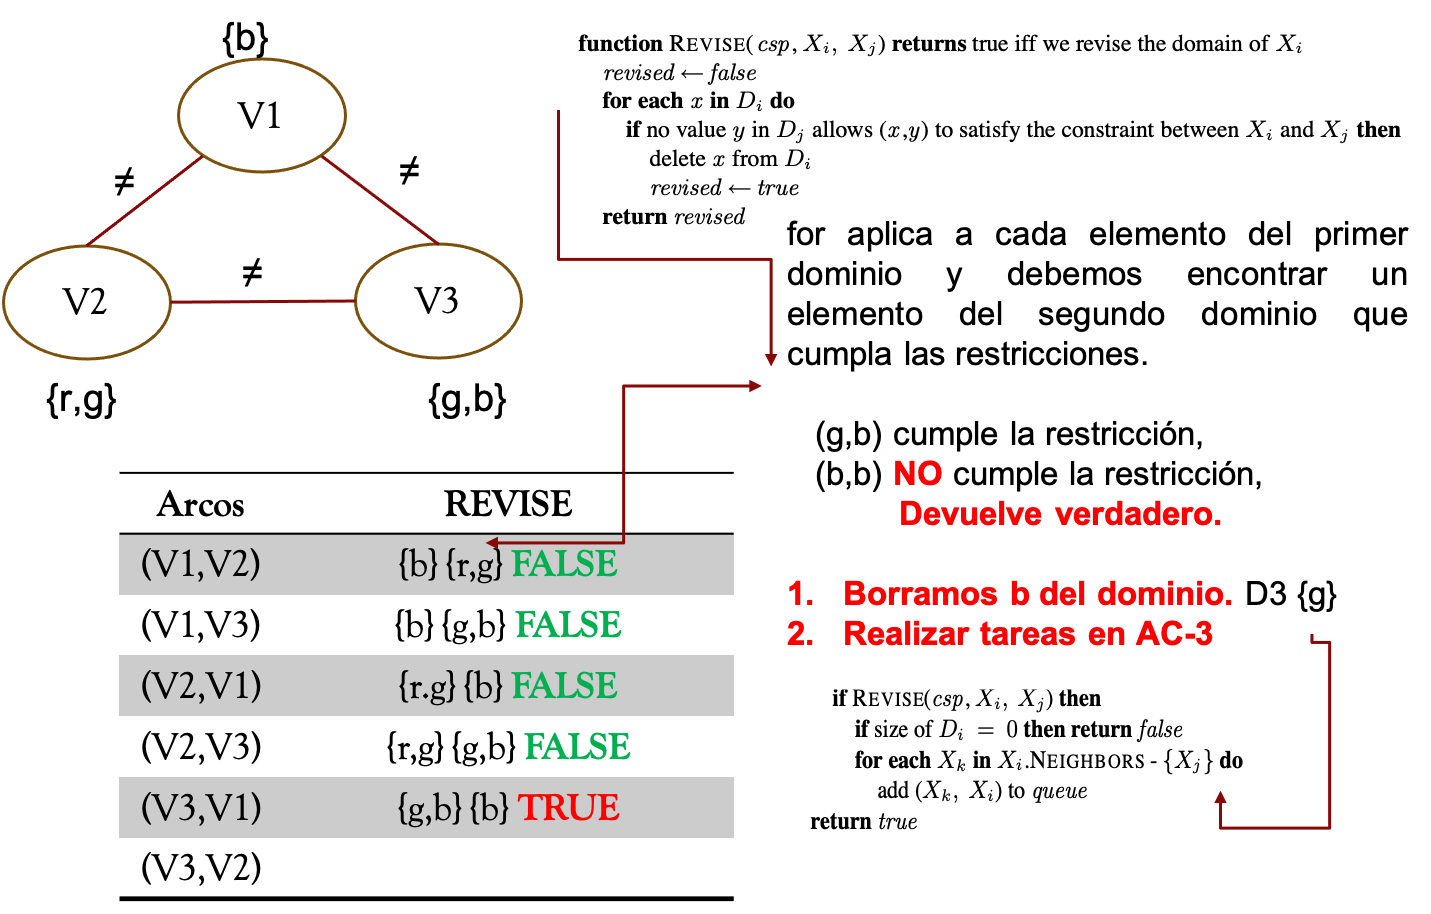
\includegraphics[scale=0.4]{./img/EjAC3_4}
\end{figure}

\end{frame} 

%%%%%%%%%%%%%%%%%%%%%%%%%%%%%%%%

\begin{frame}  \frametitle{Ejemplo Algoritmo AC-3 } \small

\begin{figure}
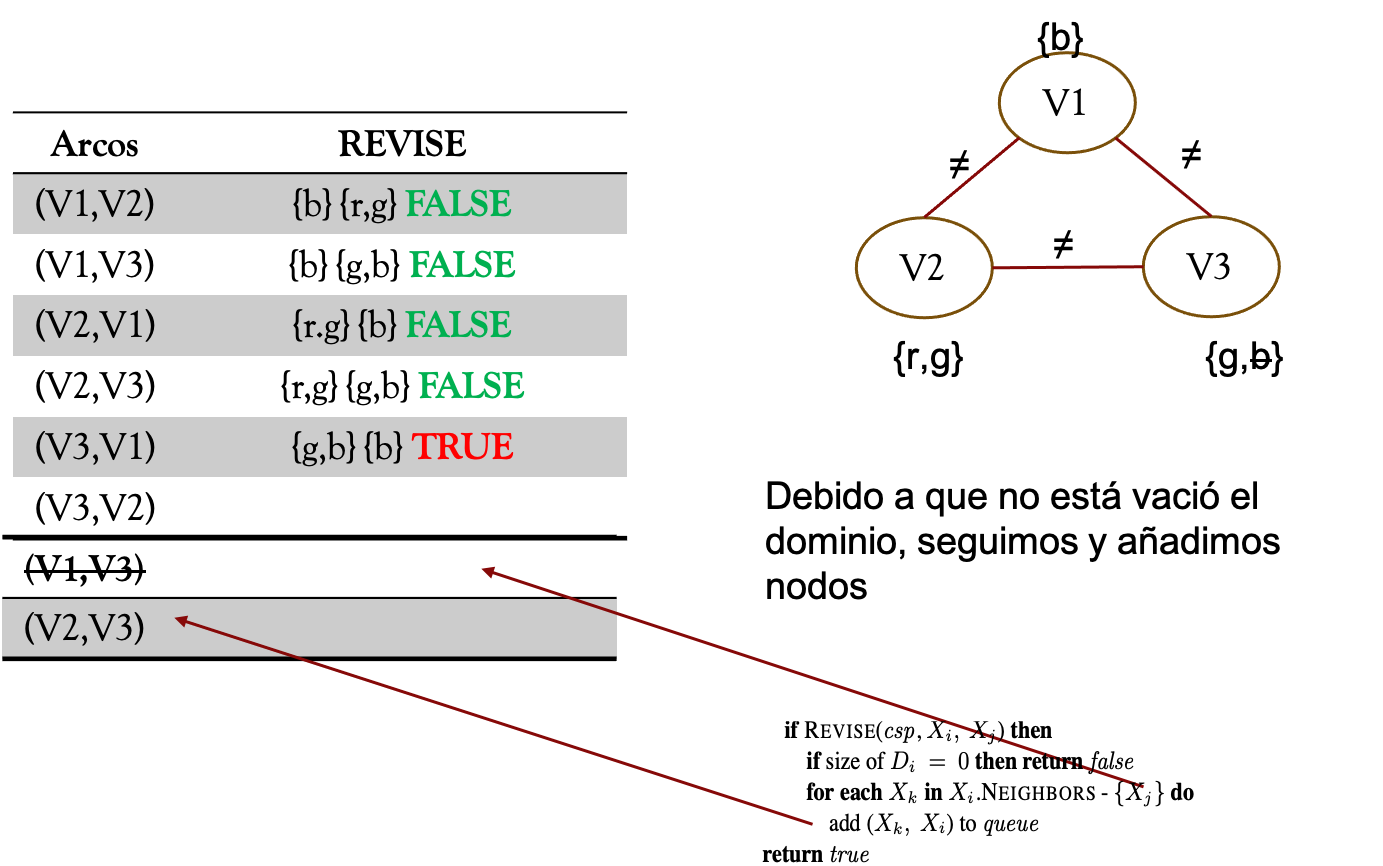
\includegraphics[scale=0.45]{./img/EjAC3_5}
\end{figure}

\end{frame} 


%%%%%%%%%%%%%%%%%%%%%%%%%%%%%%%%

\begin{frame}  \frametitle{Ejemplo Algoritmo AC-3 } \small

\begin{figure}
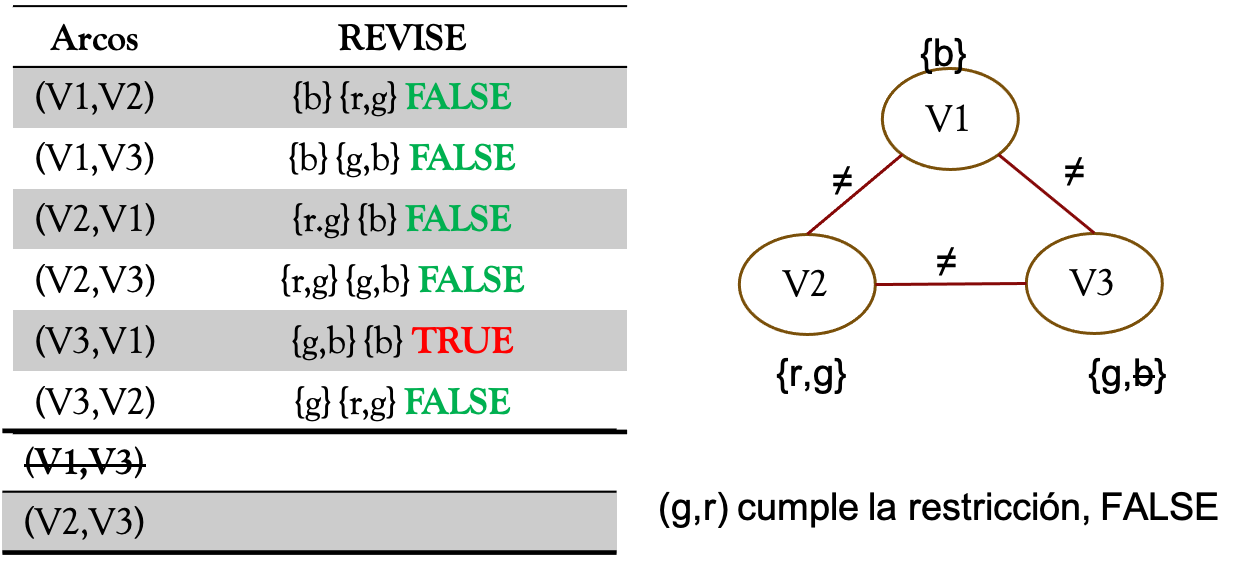
\includegraphics[scale=0.45]{./img/EjAC3_6}
\end{figure}

\end{frame} 

%%%%%%%%%%%%%%%%%%%%%%%%%%%%%%%%

\begin{frame}  \frametitle{Ejemplo Algoritmo AC-3 } \small

\begin{figure}
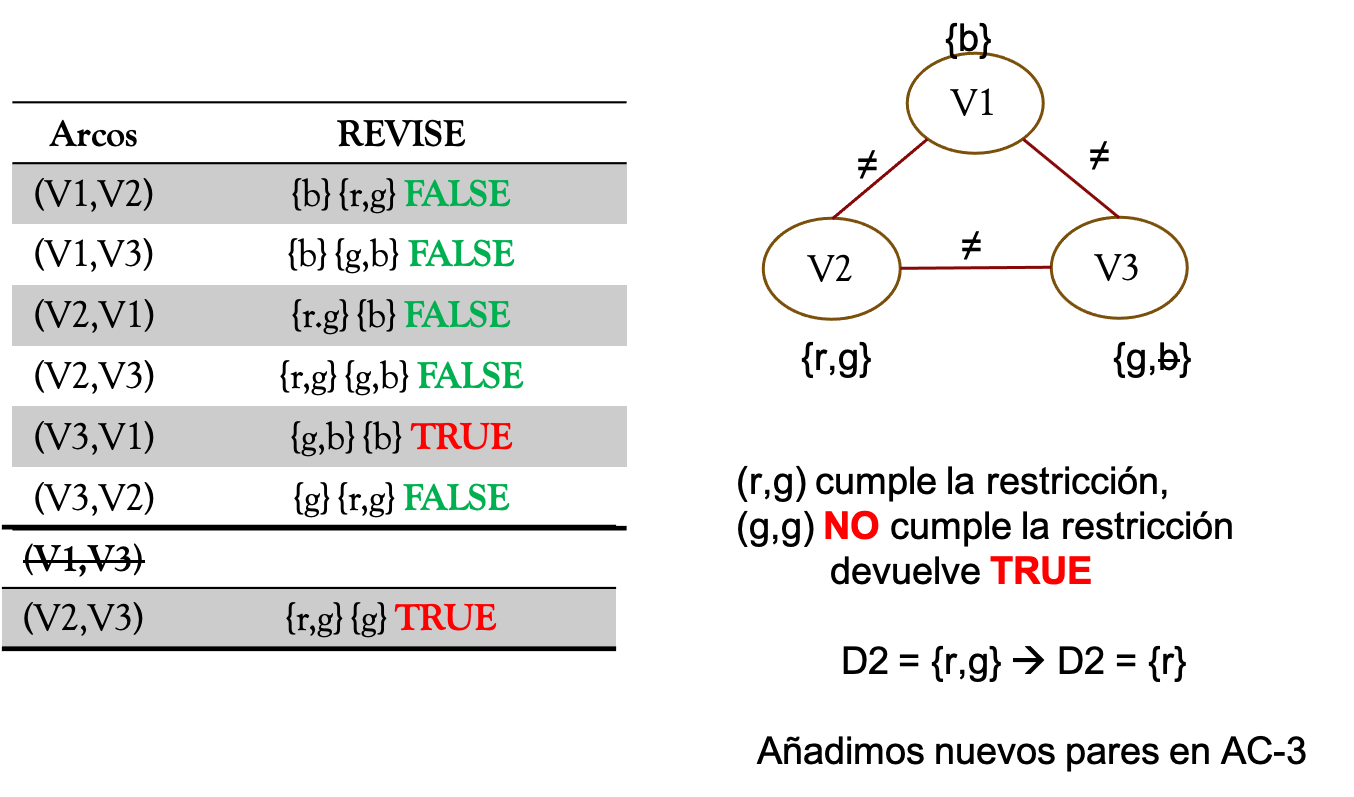
\includegraphics[scale=0.45]{./img/EjAC3_7}
\end{figure}

\end{frame} 

%%%%%%%%%%%%%%%%%%%%%%%%%%%%%%%%

\begin{frame}  \frametitle{Ejemplo Algoritmo AC-3 } \small

\begin{figure}
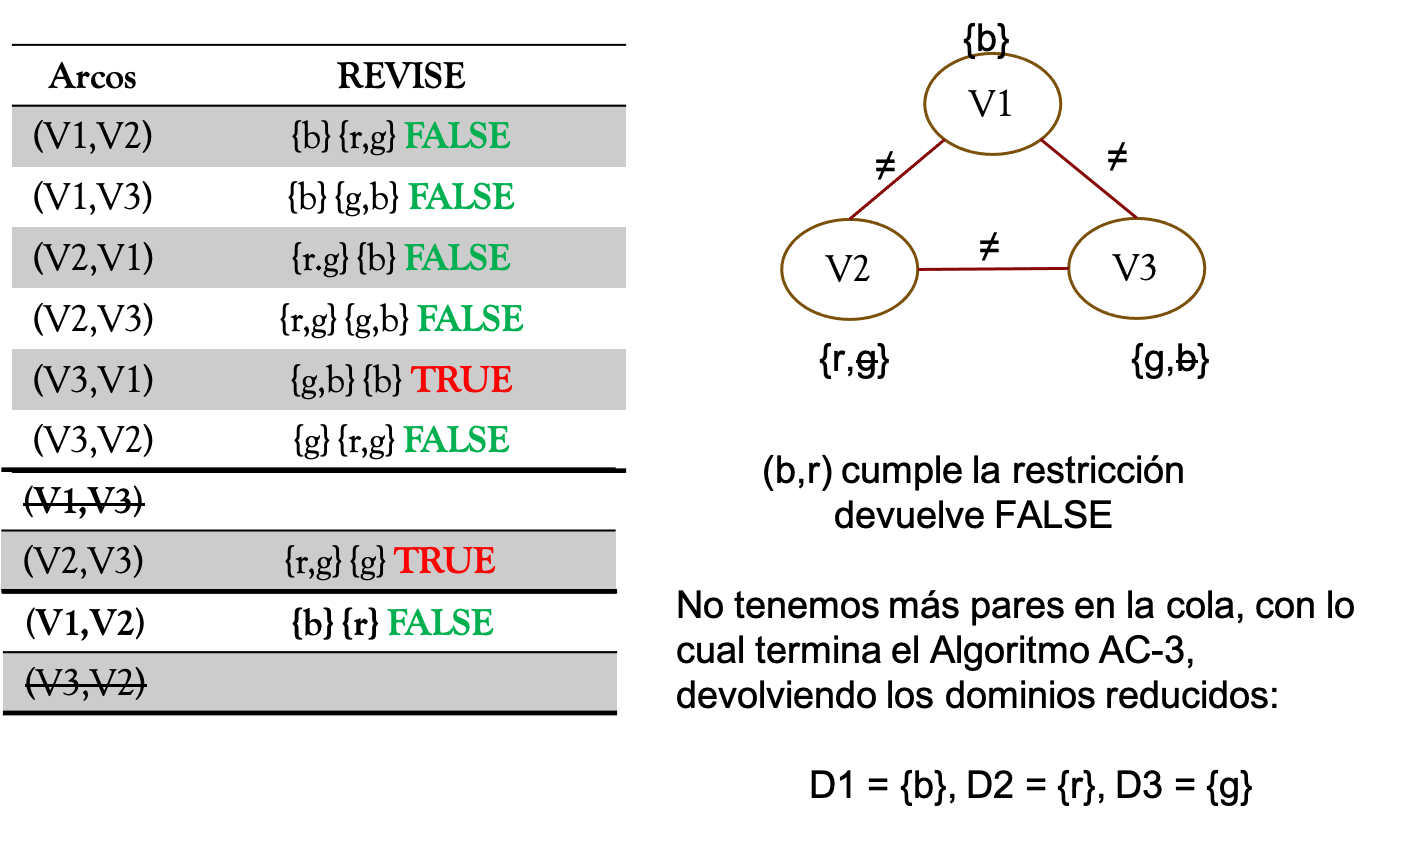
\includegraphics[scale=0.45]{./img/EjAC3_8}
\end{figure}

\end{frame} 

%%%%%%%%%%%%%%%%%%%%%%%%%%%%%%%%

\begin{frame}  \frametitle{Ejemplo 2 Algoritmo AC-3 } \small

\begin{figure}
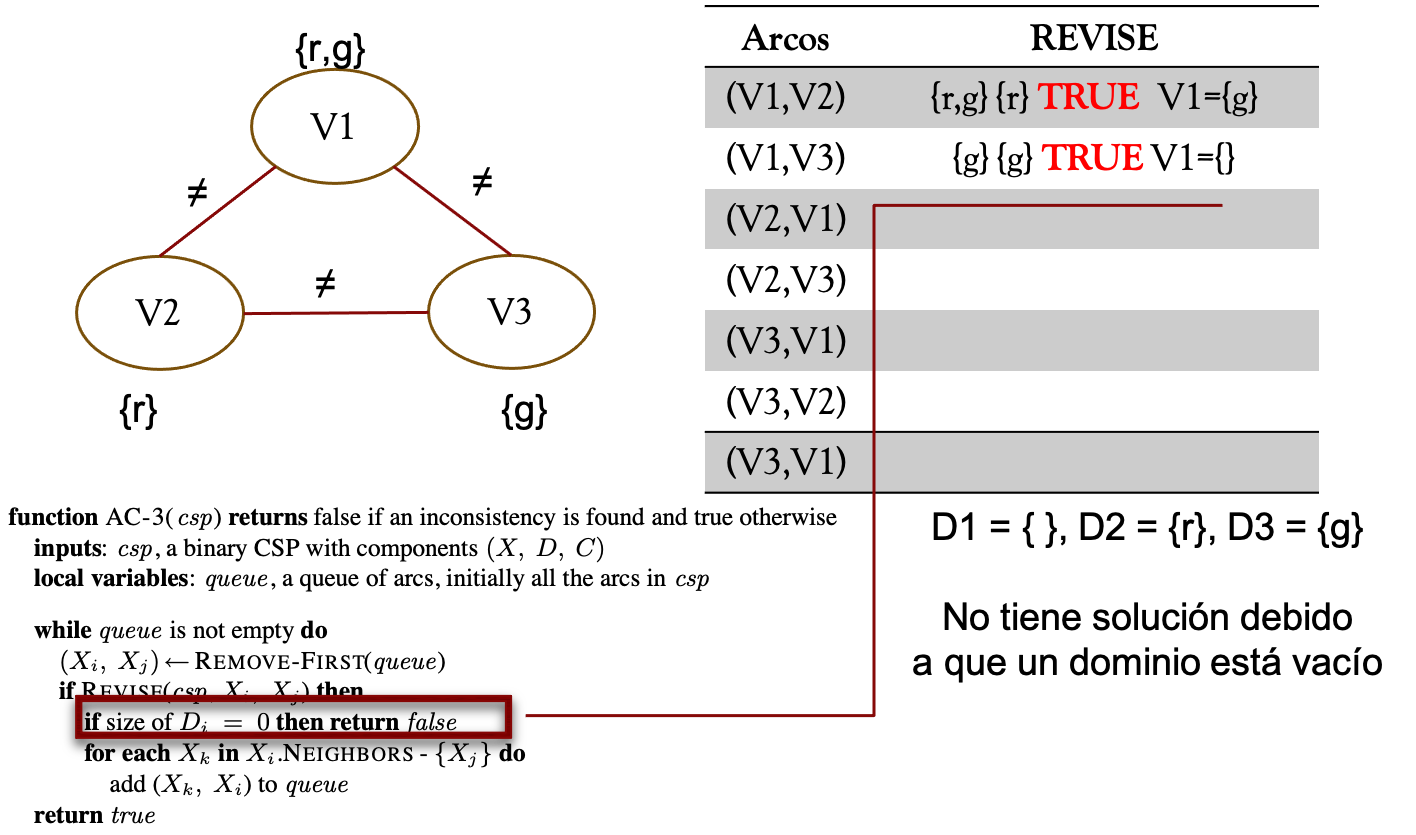
\includegraphics[scale=0.45]{./img/Ej_2AC3}
\end{figure}

\end{frame} 

%%%%%%%%%%%%%%%%%%%%%%%%%%%%%%%%

\begin{frame}  \frametitle{Ejemplo 3 Algoritmo AC-3 } \small

\begin{figure}
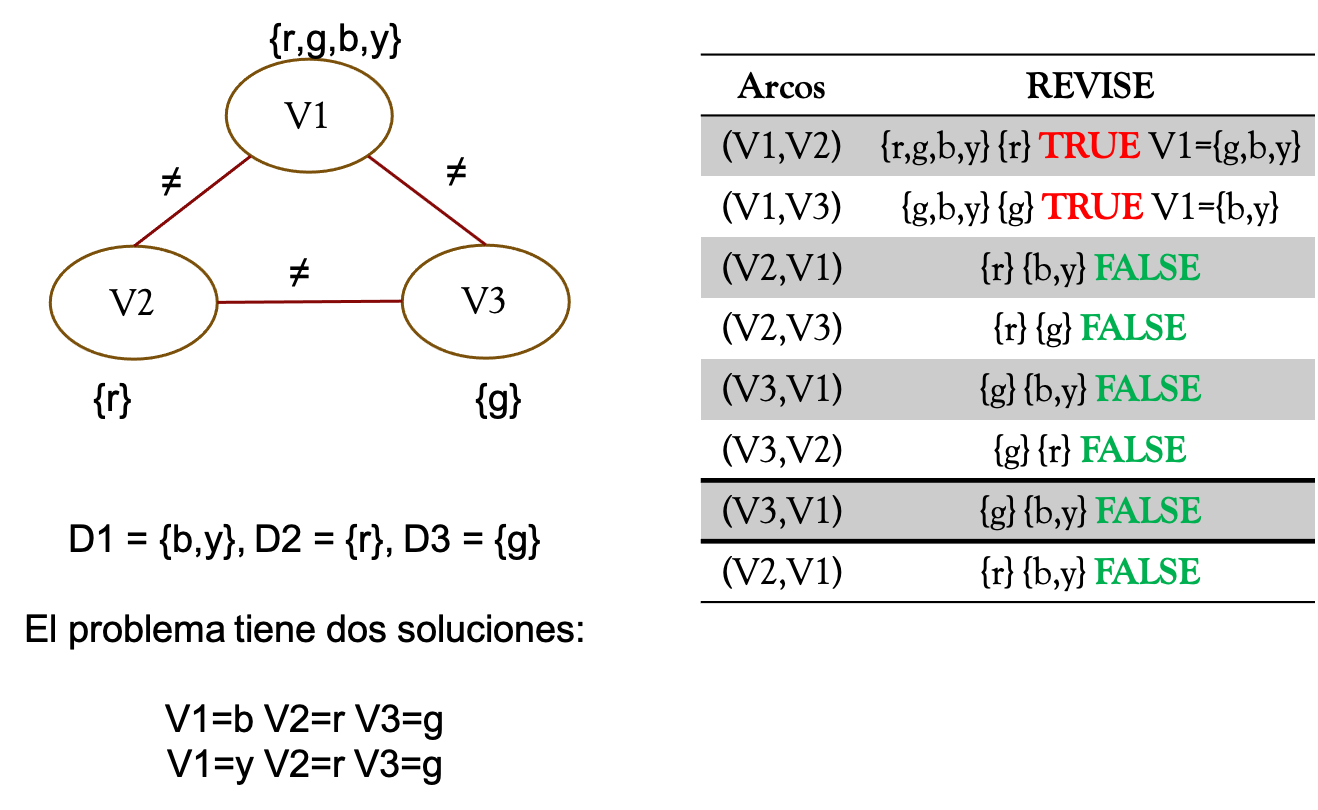
\includegraphics[scale=0.45]{./img/Ej_3AC3}
\end{figure}

\end{frame} 

%%%%%%%%%%%%%%%%%%%%%%%%%%%%%%%%
%%%%%%%%%%%%%%%%%%%%%%%%%%%%%%%%
\subsection{Ejemplo Sudoku}
%%%%%%%%%%%%%%%%%%%%%%%%%%%%%%%%

\begin{frame}  \frametitle{Sudoku} \small

\begin{figure}
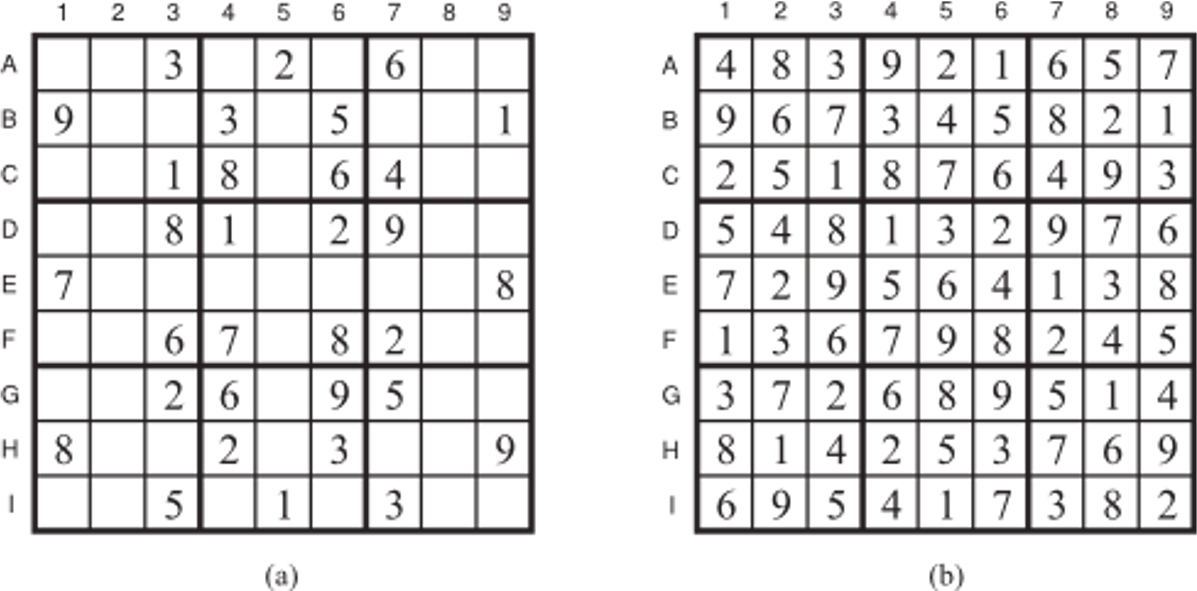
\includegraphics[scale=0.45]{./img/Sudoku}
\end{figure}

\end{frame} 

%%%%%%%%%%%%%%%%%%%%%%%%%%%%%%%%

\begin{frame}  \frametitle{Sudoku} \small

\begin{itemize}
\item Un sudoku es un CSP con 81 variables, una para cada casilla.
\item Las casillas vacías tienen un dominio \{1,2,3,4,5,6,7,8,9\}\\
Las casillas rellenas tienen un dominio con un único valor.

\item Hay 27 \textit{Alldiff} restricciones: una para cada fila, columna y casillas de 9 esquinas.

\begin{itemize}
\item Alldiff (A1,A2,A3,A4,A5,A6,A7,A8,A9)

\item Alldiff (B1,B2,B3,B4,B5,B6,B7,B8,B9)

\item Alldiff (A1,A2,A3,B1,B2,B3,C1,C2,C3)

\item $\ldots$

\end{itemize}

\end{itemize}

\end{frame} 

%%%%%%%%%%%%%%%%%%%%%%%%%%%%%%%%

\begin{frame}  \frametitle{Sudoku} \footnotesize


\begin{minipage}{0.4\textwidth}
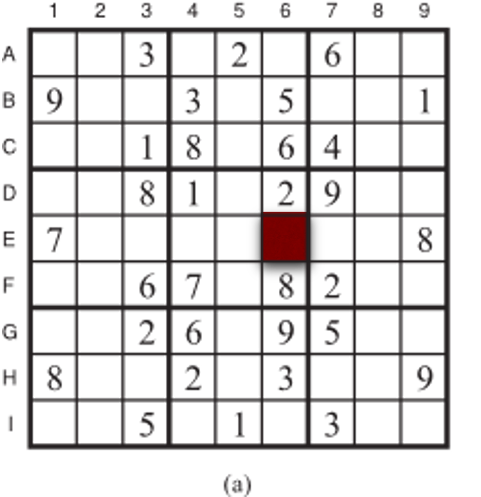
\includegraphics[scale=0.45]{./img/SudokuE6}  
\end{minipage}
\begin{minipage}{0.5\textwidth}
Consideramos variable E6.

\begin{itemize}
\item  Casillas: Podemos eliminar 1,7,2,8 del dominio. 
Dcasillas=\{3,4,5,6,9\}

\item Columna: Podemos eliminar 5,6,2,8,9,3 del dominio. 
DColumna=\{1,4,7\}

\item Fila: Podemos eliminar 7 y 8 del dominio 
DFila=\{1,2,3,4,5,6,9\}

\item Domino E6 =\{4\}
\end{itemize}

Hemos asignado el valor a la variable E6 sin tener que aplicar el algoritmo de backtracking


\end{minipage}
\end{frame} 

%%%%%%%%%%%%%%%%%%%%%%%%%%%%%%%%

\begin{frame}  \frametitle{Sudoku} \footnotesize


\begin{minipage}{0.4\textwidth}
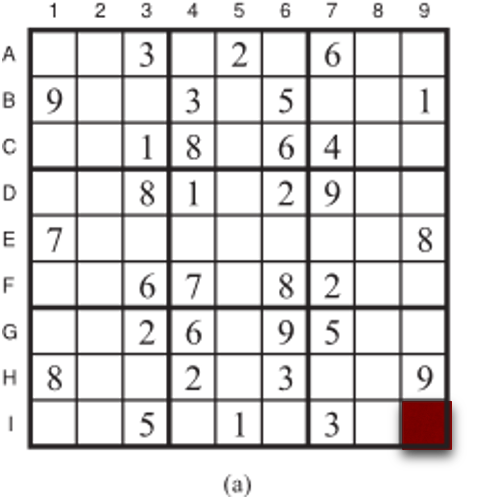
\includegraphics[scale=0.45]{./img/SudokuI9}  
\end{minipage}
\begin{minipage}{0.5\textwidth}
Consideramos variable I9.

\begin{itemize}
\item  Casillas: Podemos eliminar 3,5,9 del dominio. 
DI9=\{1,2,4,6,7,8\}

\item Columna: Podemos eliminar 1,8,9 del dominio.  
DI9=\{2,4,6,7\}

\item Fila: Podemos eliminar 1,5,3 del dominio
 DI9=\{2,4,6,7\}

\item DominoI9 =\{2,4,6,7\}
\end{itemize}

En este caso no podemos asignar el valor a a la variable I9, con lo cual deberemos hacer uso del algoritmo de backtracking.

\end{minipage}
\end{frame} 

\section{Algoritmos}
%%%%%%%%%%%%%%%%%%%%%%%%%%%%%%%%
%%%%%%%%%%%%%%%%%%%%%%%%%%%%%%%%

\subsection{Vuelta Atrás}
%%%%%%%%%%%%%%%%%%%%%%%%%%%%%%%%
%%%%%%%%%%%%%%%%%%%%%%%%%%%%%%%%


\begin{frame}  \frametitle{Algoritmo vuelta atrás} \footnotesize

\begin{itemize}
\item Muchos CSPs no se pueden resolver solamente por inferencia sobre las restricciones; llega un momento en el que hay que buscar una solución
\item  La búsqueda por vuelta atrás es una búsqueda primero en profundidad que en cada momento elige un valor para una sola variable, 

y vuelve atrás cuando una variable no tiene ningún valor legal que quede por probar

\item  Debemos considerar las siguientes preguntas:
\begin{enumerate}
\item ¿Qué variable debería ser asignada a continuación?
\item ¿En qué orden deberíamos probar sus valores?
\item ¿Qué inferencias deberían realizarse en cada paso?
\end{enumerate}

\end{itemize}


\end{frame} 

%%%%%%%%%%%%%%%%%%%%%%%%%%%%%%%%

\begin{frame}  \frametitle{Algoritmo vuelta atrás} \footnotesize

\begin{figure}
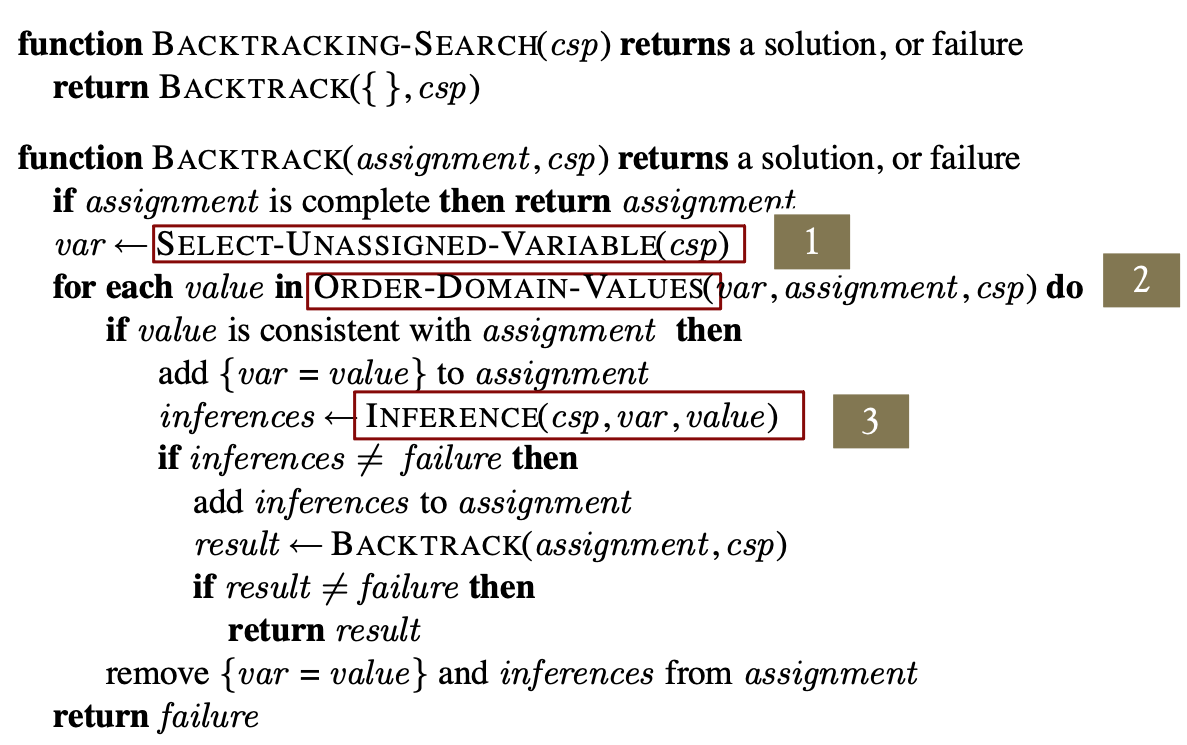
\includegraphics[scale=0.45]{./img/Alg_Back}
\end{figure}


\end{frame} 

%%%%%%%%%%%%%%%%%%%%%%%%%%%%%%%%


\begin{frame}  \frametitle{Ejemplo Algoritmo vuelta atrás} \footnotesize

\begin{figure}
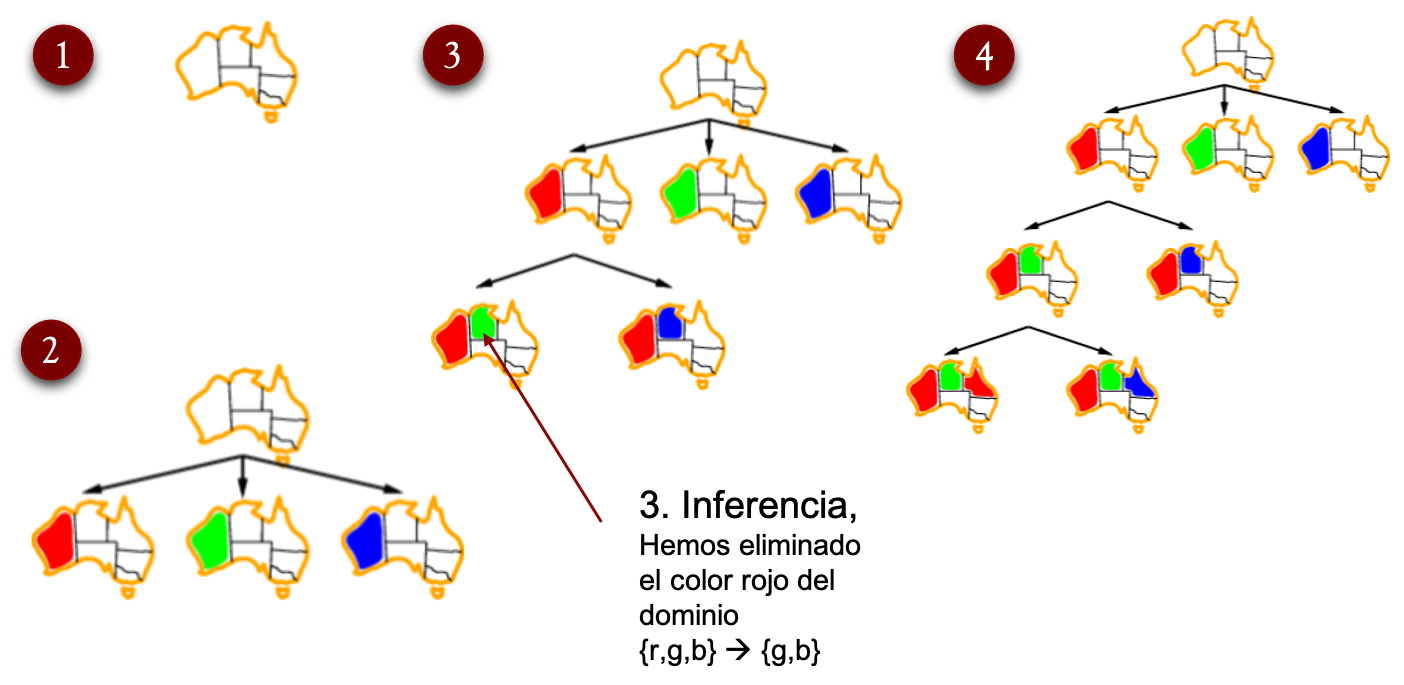
\includegraphics[scale=0.45]{./img/Alg_Back_Australia}
\end{figure}


\end{frame} 


%%%%%%%%%%%%%%%%%%%%%%%%%%%%%%%%


\begin{frame}  \frametitle{1. Ordenación de las variables} \footnotesize

\begin{itemize}
\item Habitualmente se elige la variable que tenga el menor número de valores legales. Esto es lo que se llama el heurístico del mínimo número de valores restantes.                                              			 	

\begin{center}
(minimum remaining values heuristic, MRV)
\end{center}

\begin{center}
WA = {red,green,blue},  Q ={red}
\end{center}
	
\item También es posible emplear el heurístico del grado (degree heuristic, DEG), que elige la variable que interviene en el mayor número de restricciones con otras variables no asignadas.


Esta manera de elegir las variables intenta obtener un fallo tan pronto como sea posible para podar secciones más grandes del árbol de búsqueda rápidamente

\end{itemize}

\begin{figure}
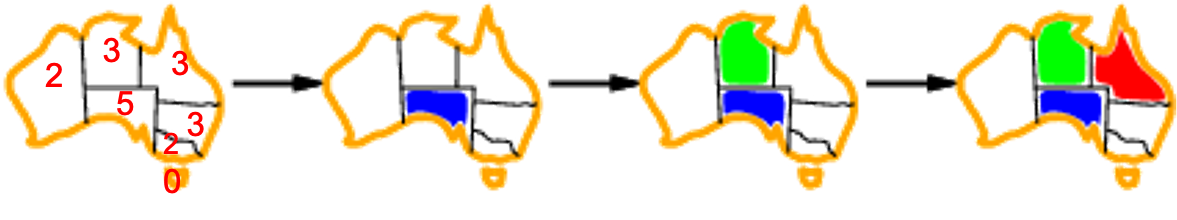
\includegraphics[scale=0.35]{./img/OrdenVariables}
\end{figure}


\end{frame} 

%%%%%%%%%%%%%%%%%%%%%%%%%%%%%%%%


\begin{frame}  \frametitle{2.Ordenación de los valores} \footnotesize


En algunos casos el heurístico del valor menos restrictivo (least constraining value, LCV) puede resultar útil

\begin{itemize}
\item Prefiere el valor que elimina el menor número de opciones para las variables vecinas en el grafo de restricciones
\item Este heurístico intenta obtener una solución tan pronto como sea posible eligiendo primero los valores más verosímiles
\end{itemize}

\begin{figure}
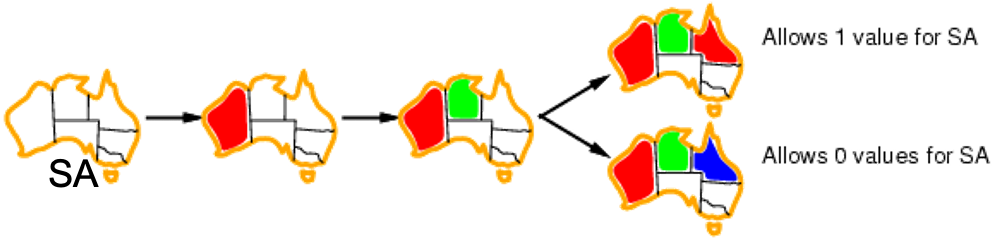
\includegraphics[scale=0.35]{./img/OrdenValores}
\end{figure}


\end{frame} 

%%%%%%%%%%%%%%%%%%%%%%%%%%%%%%%%
\begin{frame}  \frametitle{3. Intercalando búsqueda e inferencias} \footnotesize


\begin{itemize}
\item Cada vez que hacemos una elección de un valor para una variable, intentamos inferir nuevas reducciones de dominio en las variables vecinas
\item Una de las estrategias más sencillas es la comprobación hacia delante (forward checking)

Cada vez que se asigna una variable X, para cada variable no asignada Y que está conectada a X mediante una restricción, borramos del dominio de Y los valores que son inconsistentes con el valor elegido para X
\item Para muchos problemas la búsqueda es más efectiva si combinamos la heurística MRV con la comprobación hacia delante.

\item Este heurístico intenta obtener una solución tan pronto como sea posible eligiendo primero los valores más verosímiles
\end{itemize}


\end{frame} 

%%%%%%%%%%%%%%%%%%%%%%%%%%%%%%%%
\begin{frame}  \frametitle{3. Intercalando búsqueda e inferencias} \footnotesize


\begin{figure}
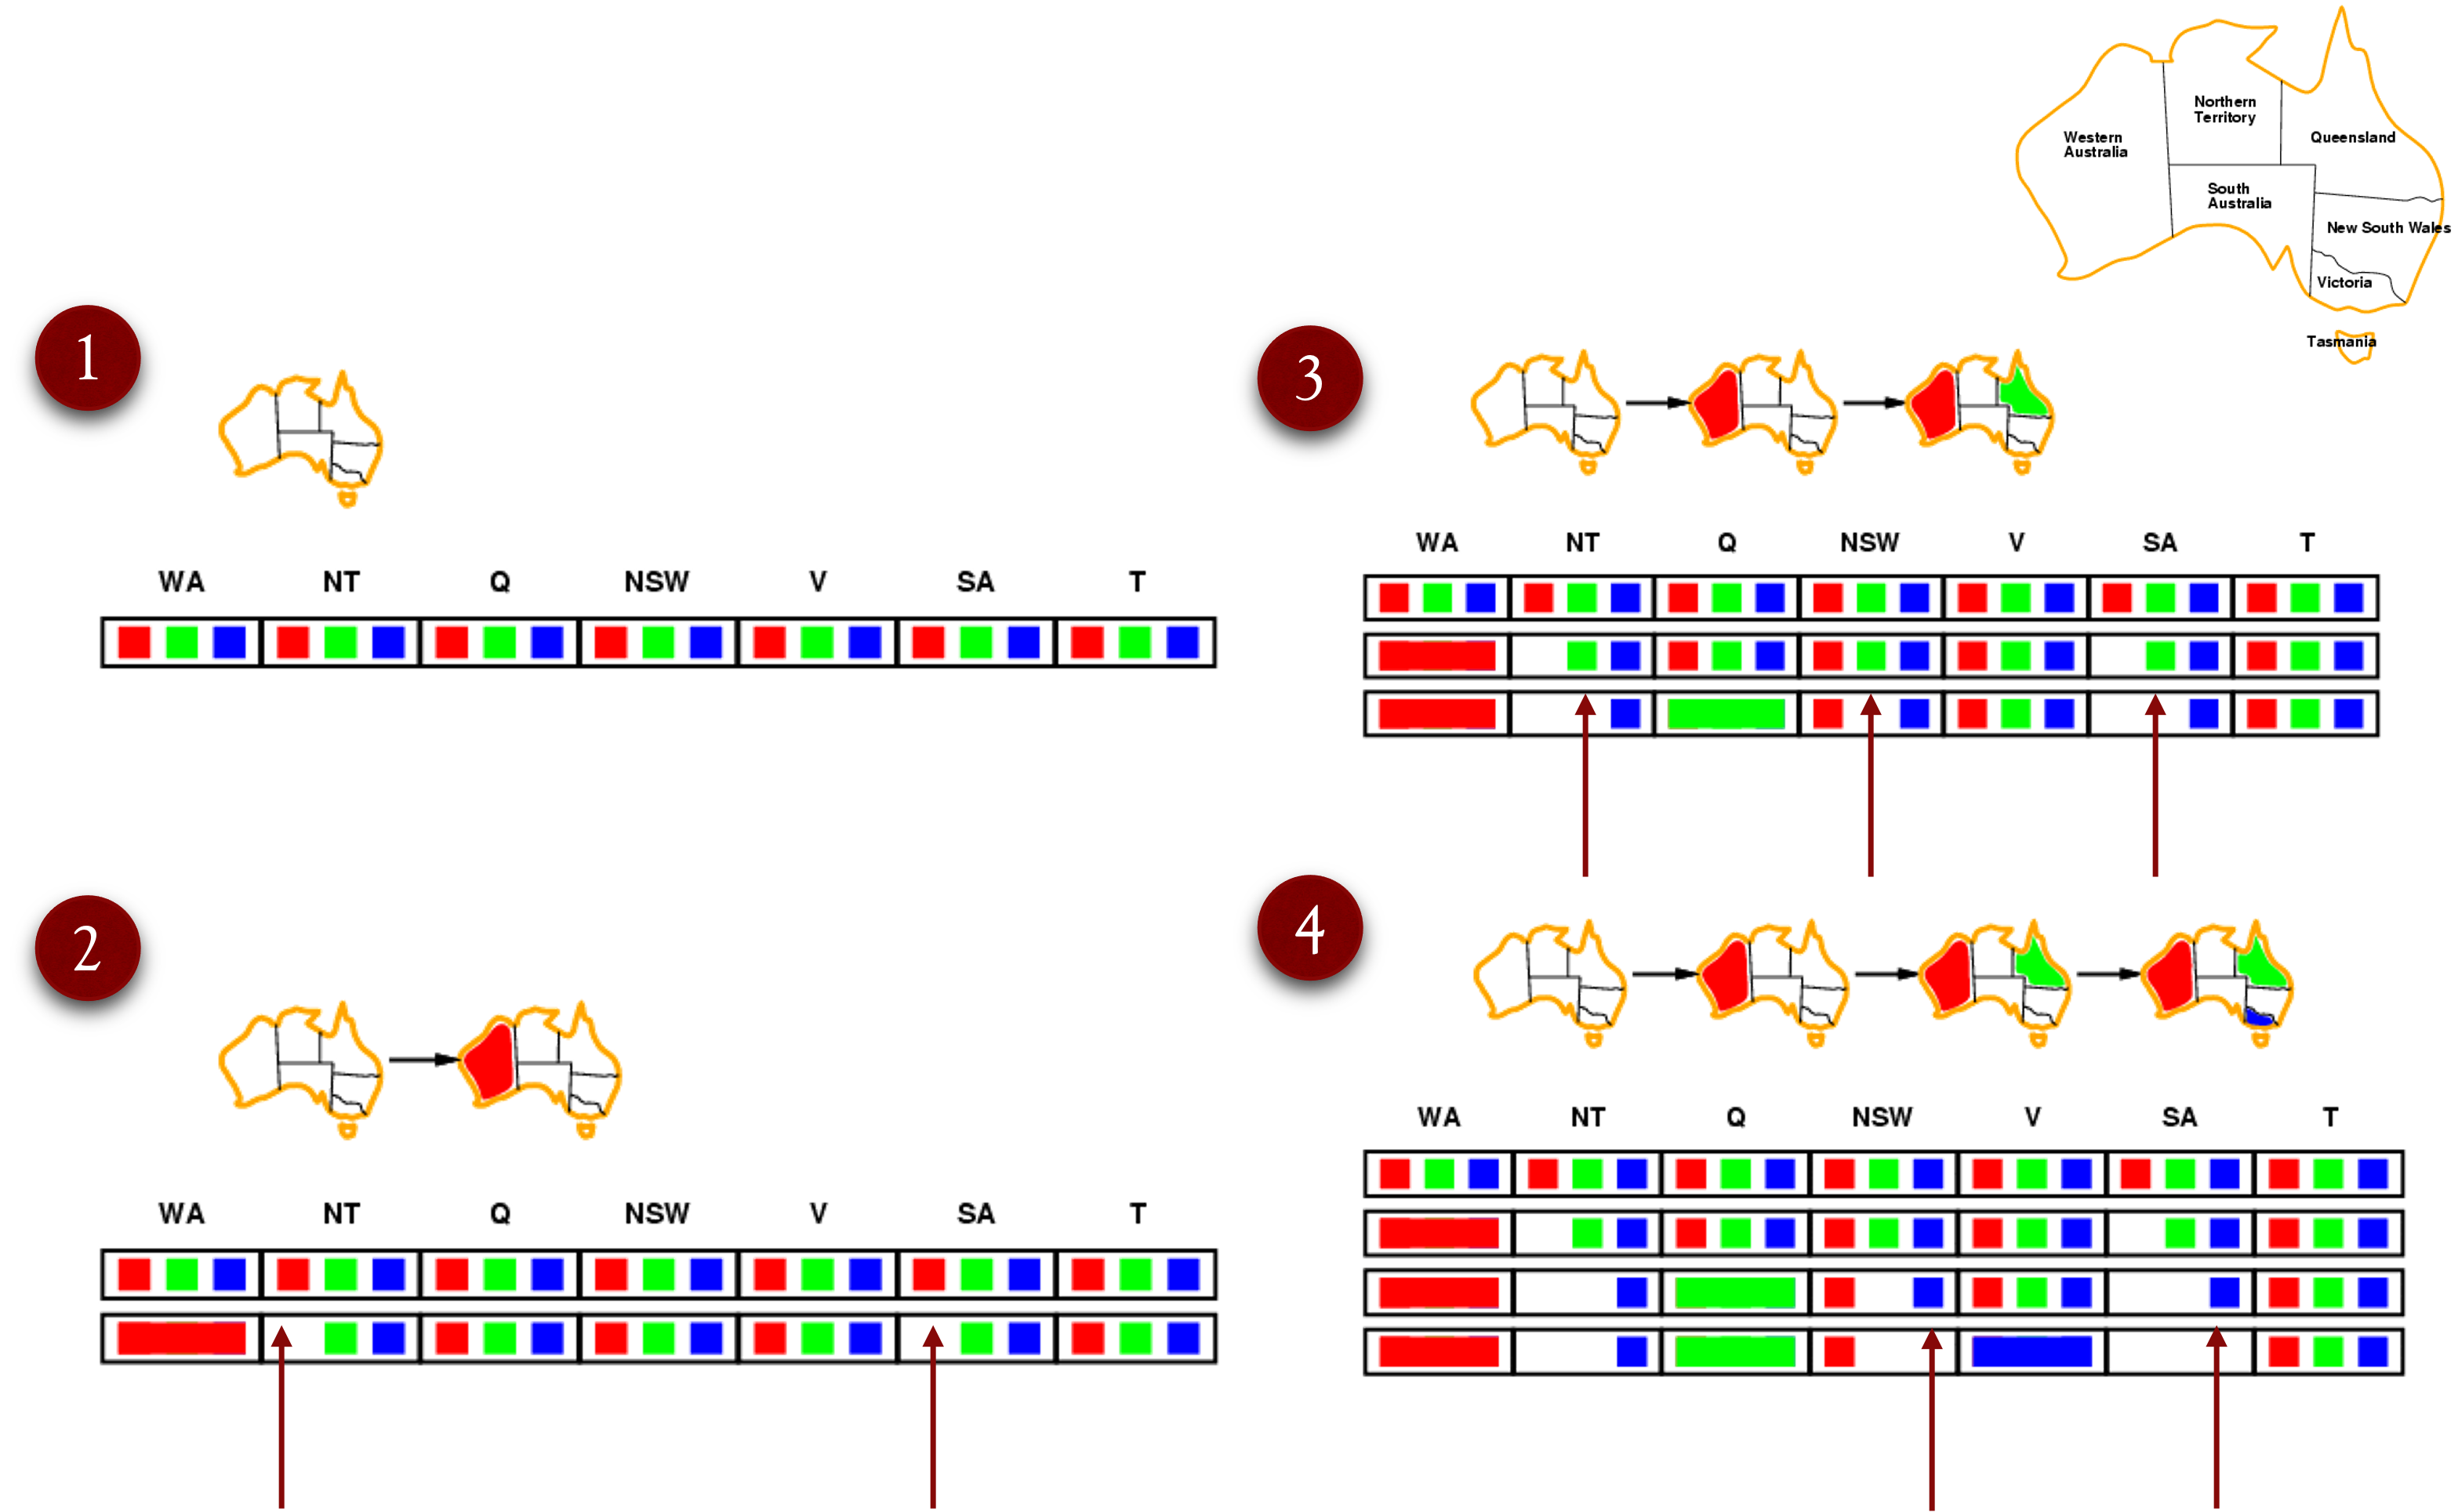
\includegraphics[scale=0.45]{./img/FC}
\end{figure}

\end{frame} 

%%%%%%%%%%%%%%%%%%%%%%%%%%%%%%%%
\begin{frame}  \frametitle{3. Intercalando búsqueda e inferencias} \footnotesize


\begin{figure}
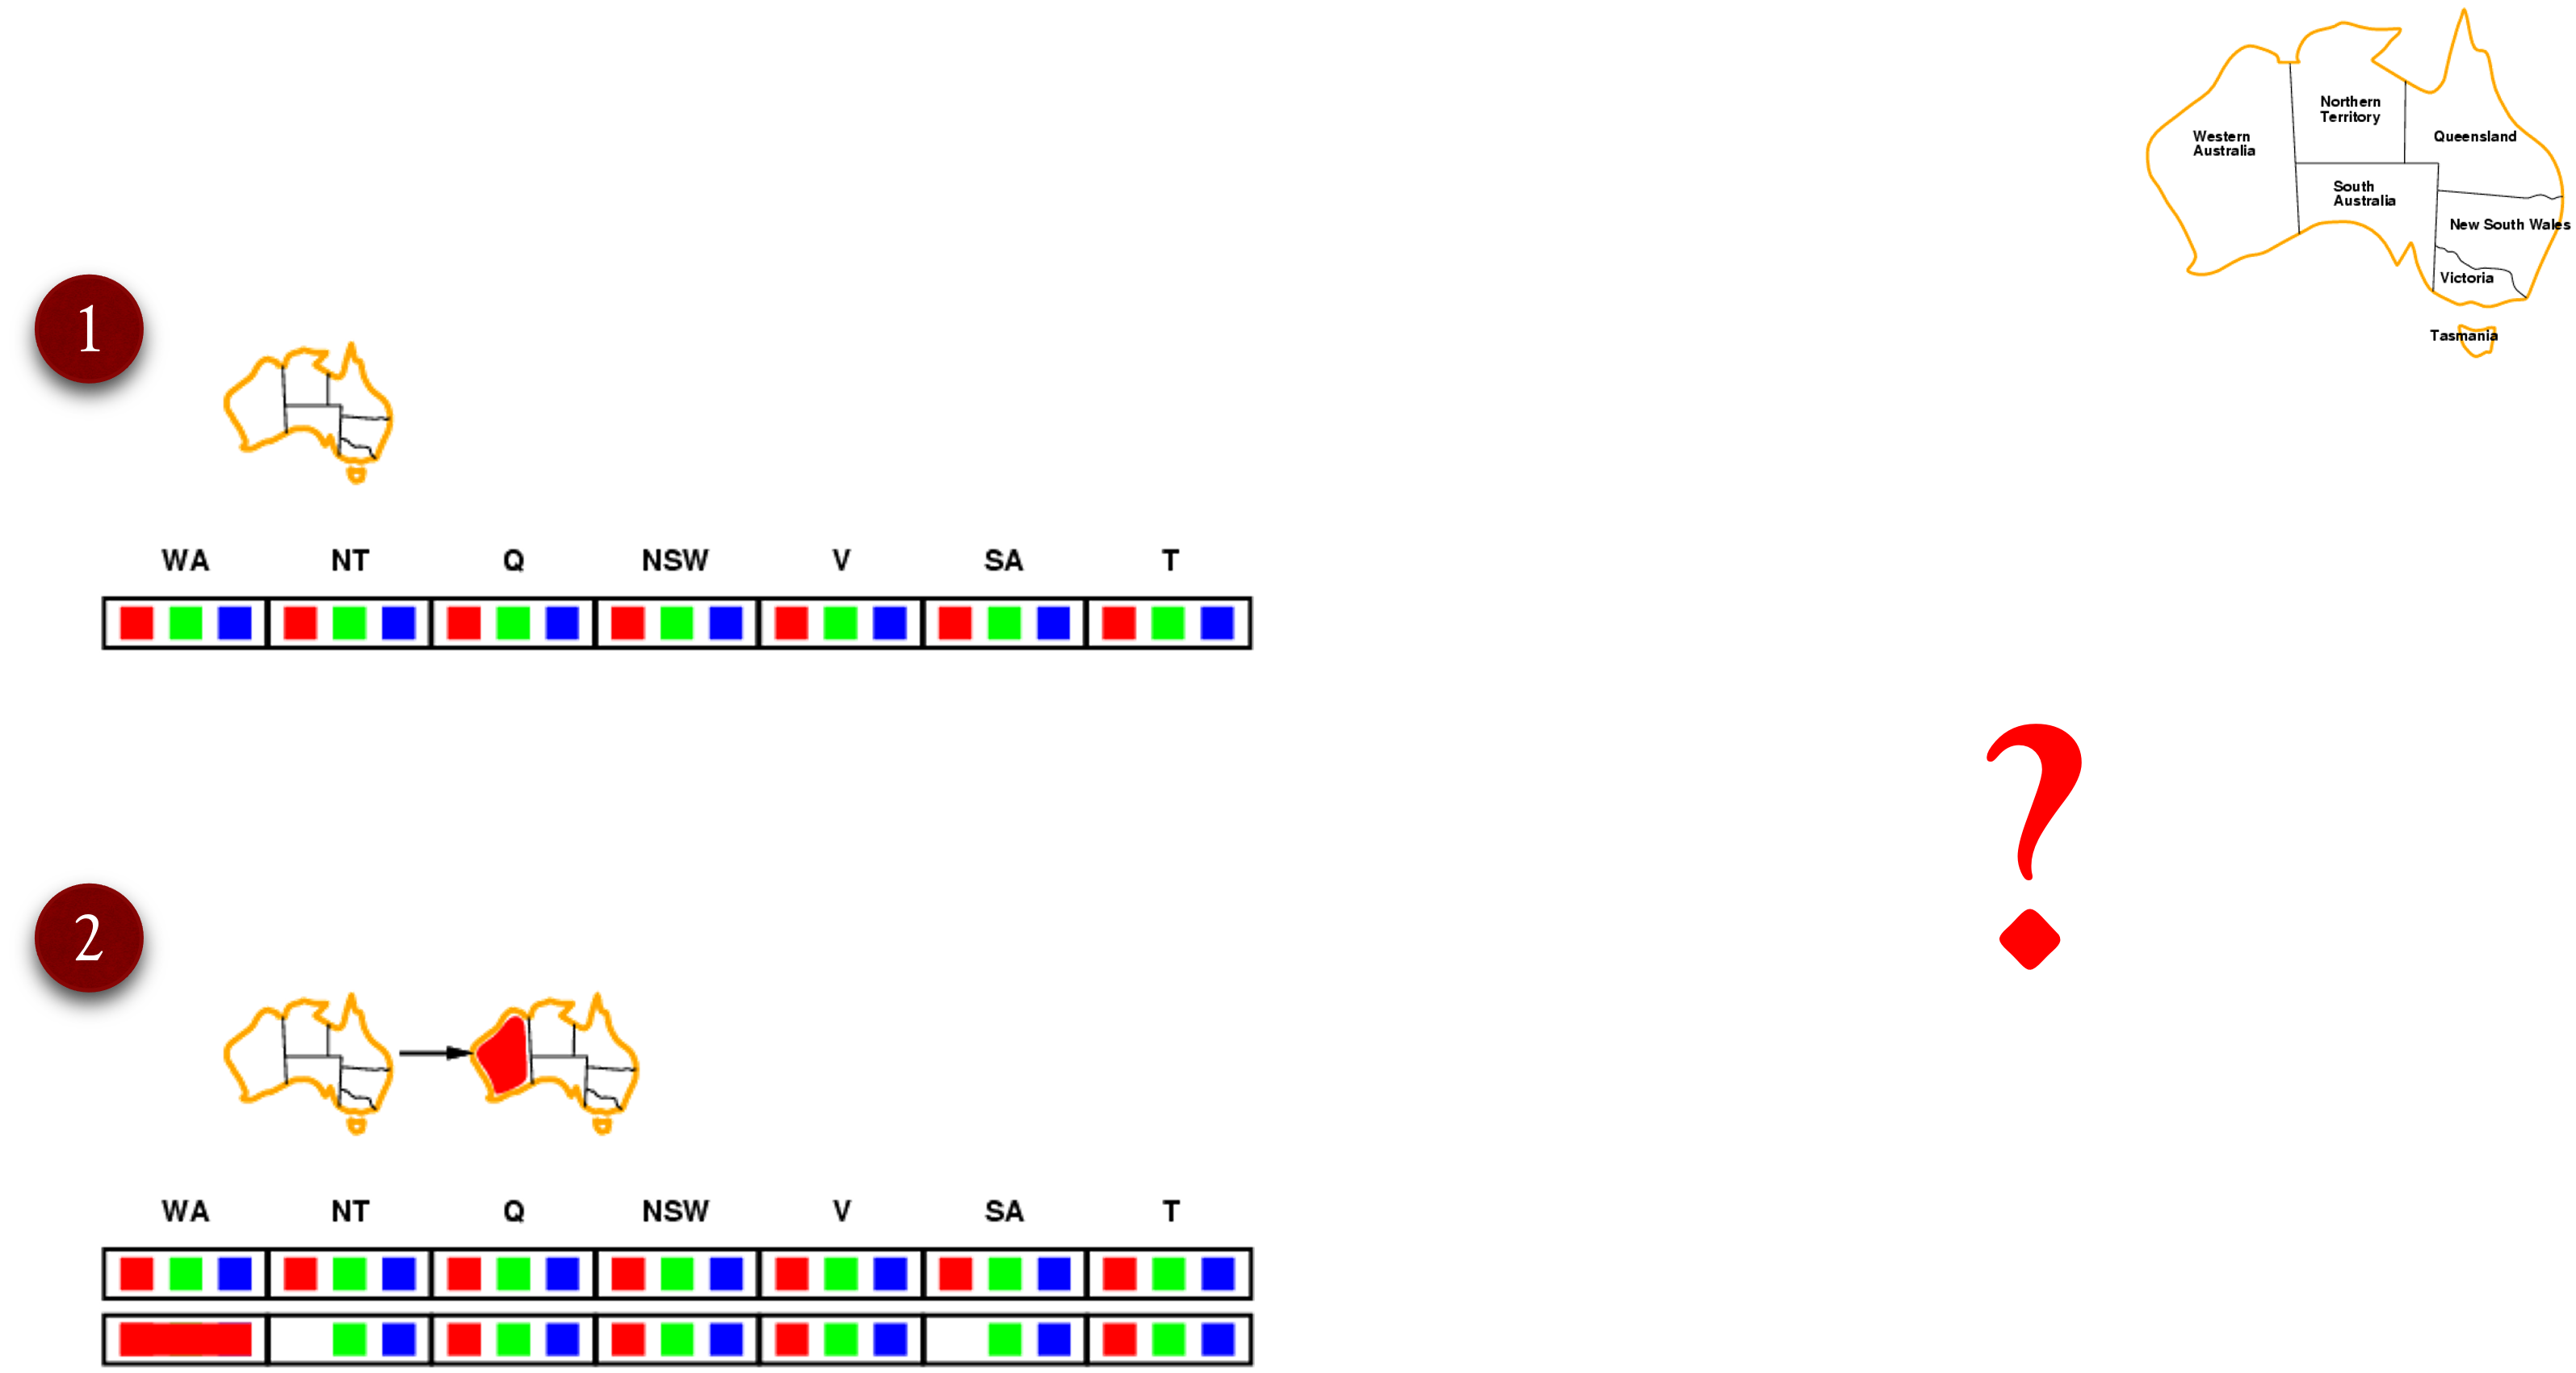
\includegraphics[scale=0.45]{./img/FC_MRV}
\end{figure}

\end{frame} 

%%%%%%%%%%%%%%%%%%%%%%%%%%%%%%%%
\begin{frame}  \frametitle{3. Intercalando búsqueda e inferencias} \footnotesize


\begin{figure}
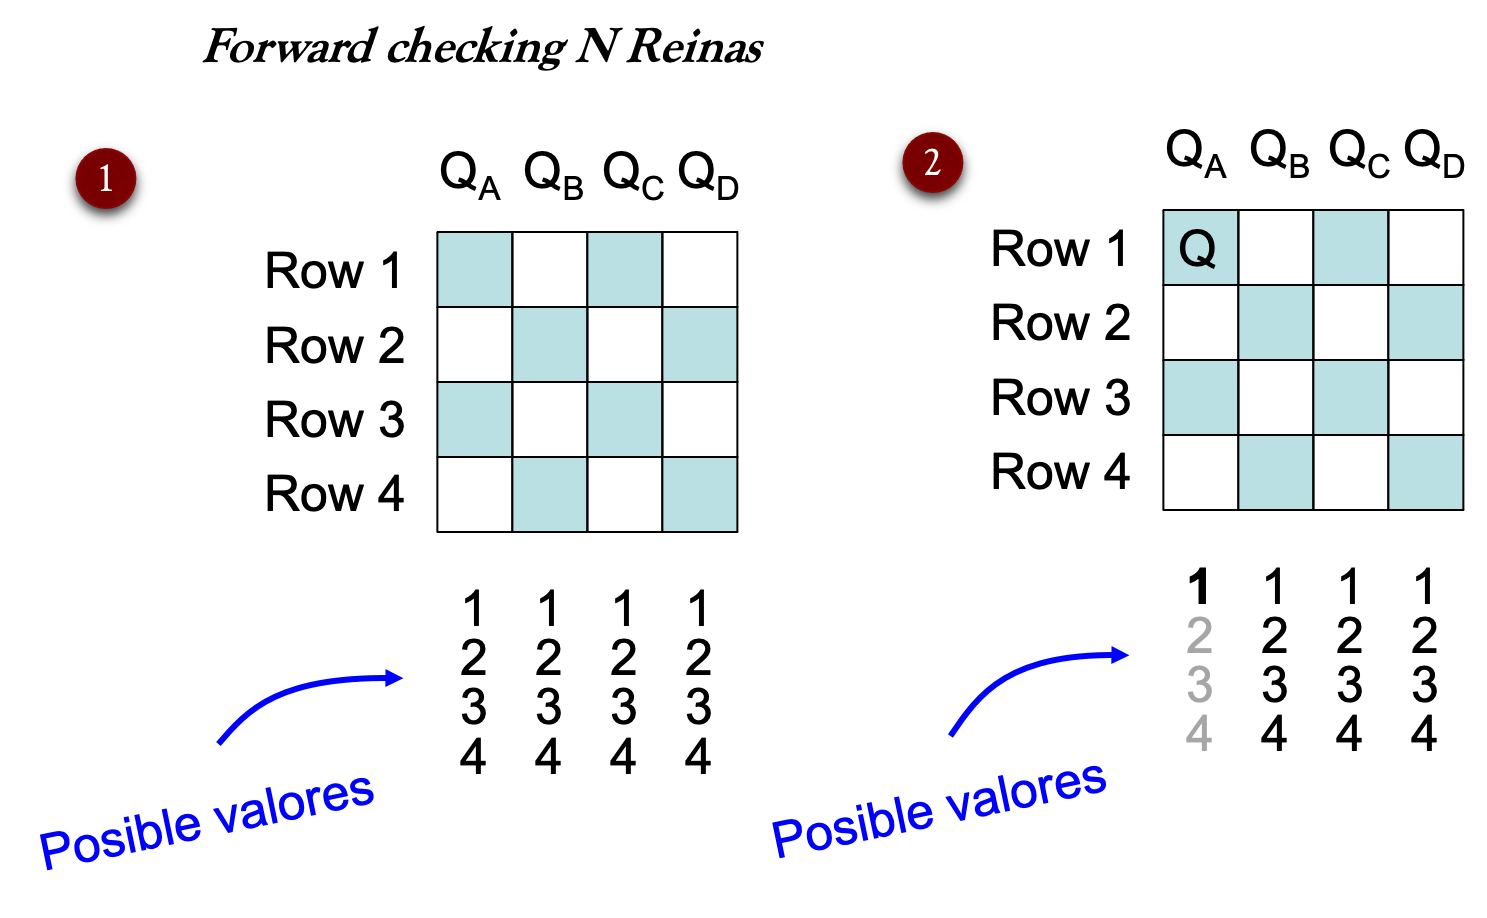
\includegraphics[scale=0.4]{./img/FC_NReinas_1}
\end{figure}

\end{frame} 

%%%%%%%%%%%%%%%%%%%%%%%%%%%%%%%%
\begin{frame}  \frametitle{3. Intercalando búsqueda e inferencias} \footnotesize


\begin{figure}
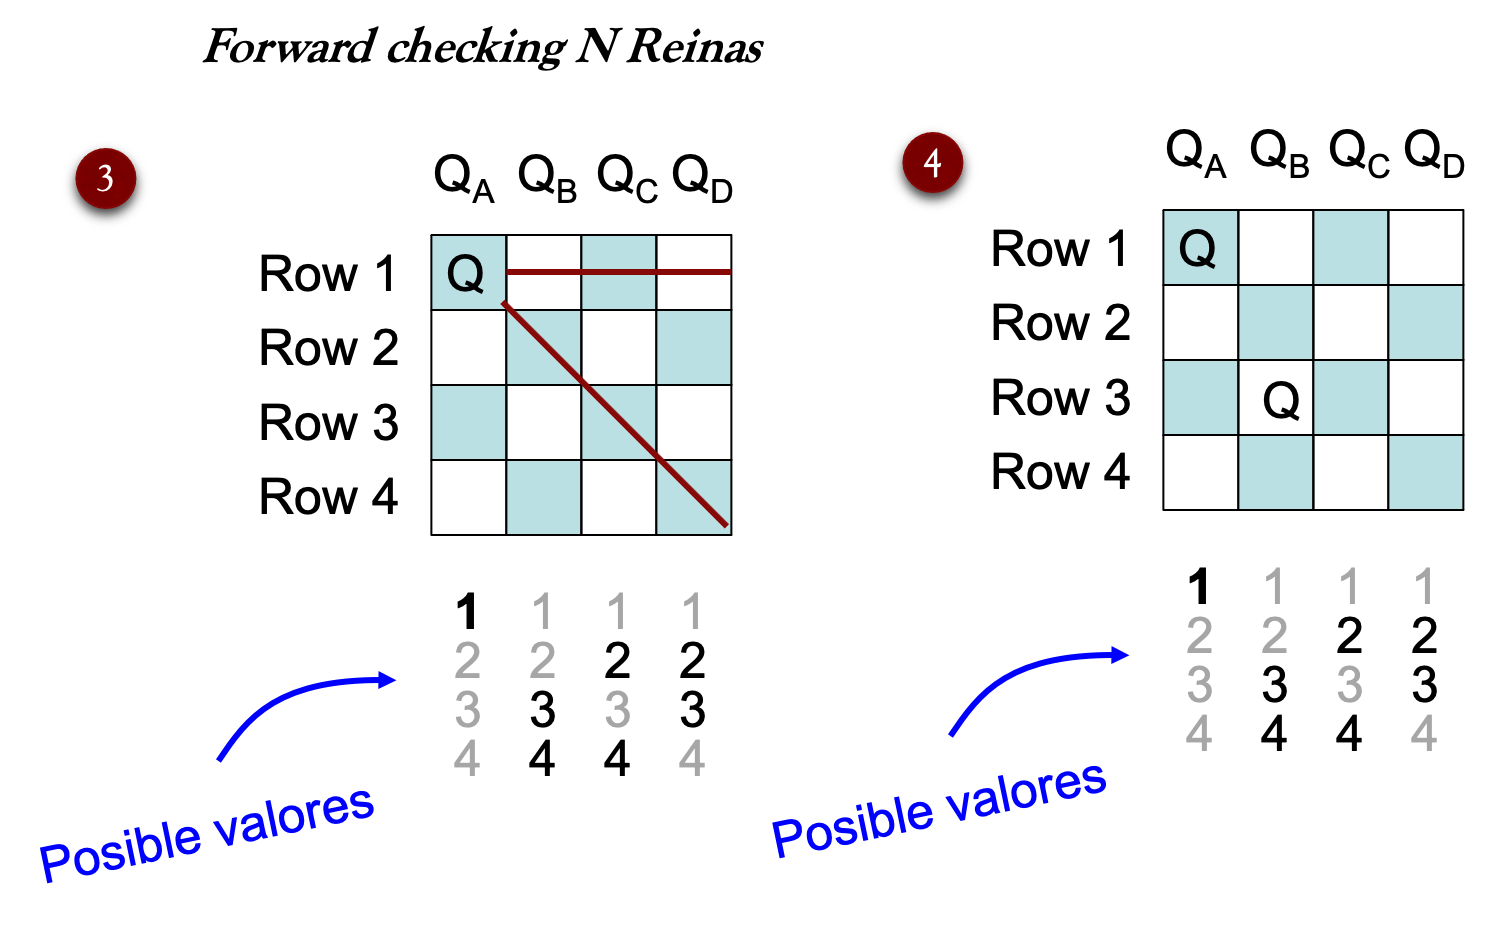
\includegraphics[scale=0.4]{./img/FC_NReinas_2}
\end{figure}

\end{frame} 


%%%%%%%%%%%%%%%%%%%%%%%%%%%%%%%%
\begin{frame}  \frametitle{3. Intercalando búsqueda e inferencias} \footnotesize


\begin{figure}
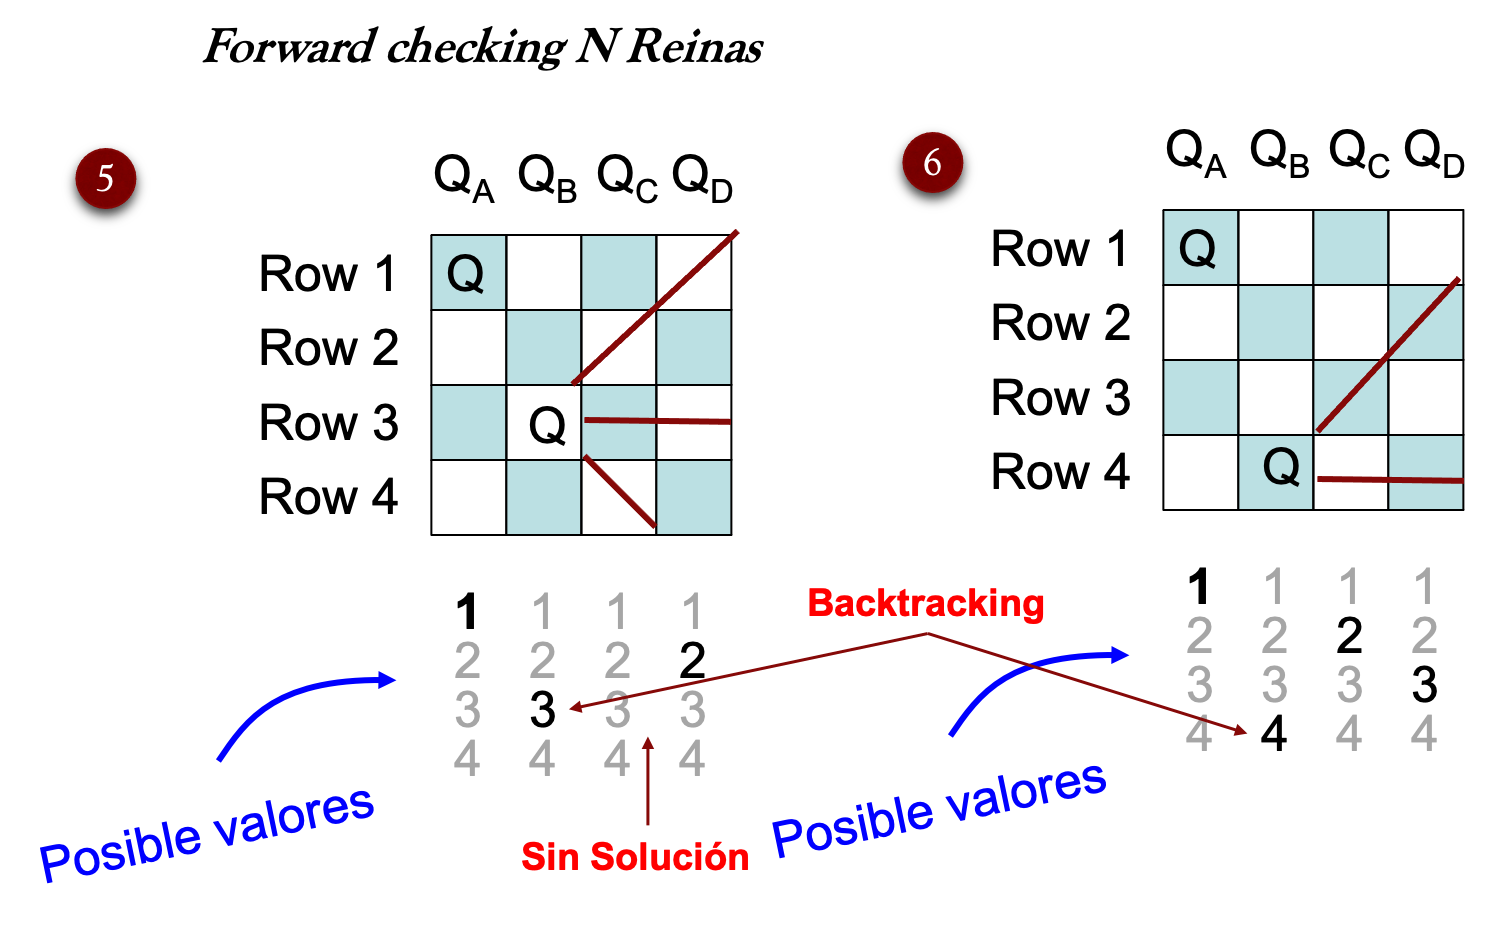
\includegraphics[scale=0.4]{./img/FC_NReinas_3}
\end{figure}

\end{frame} 

%%%%%%%%%%%%%%%%%%%%%%%%%%%%%%%%
\begin{frame}  \frametitle{Backtracking N Reinas} \footnotesize


\begin{figure}
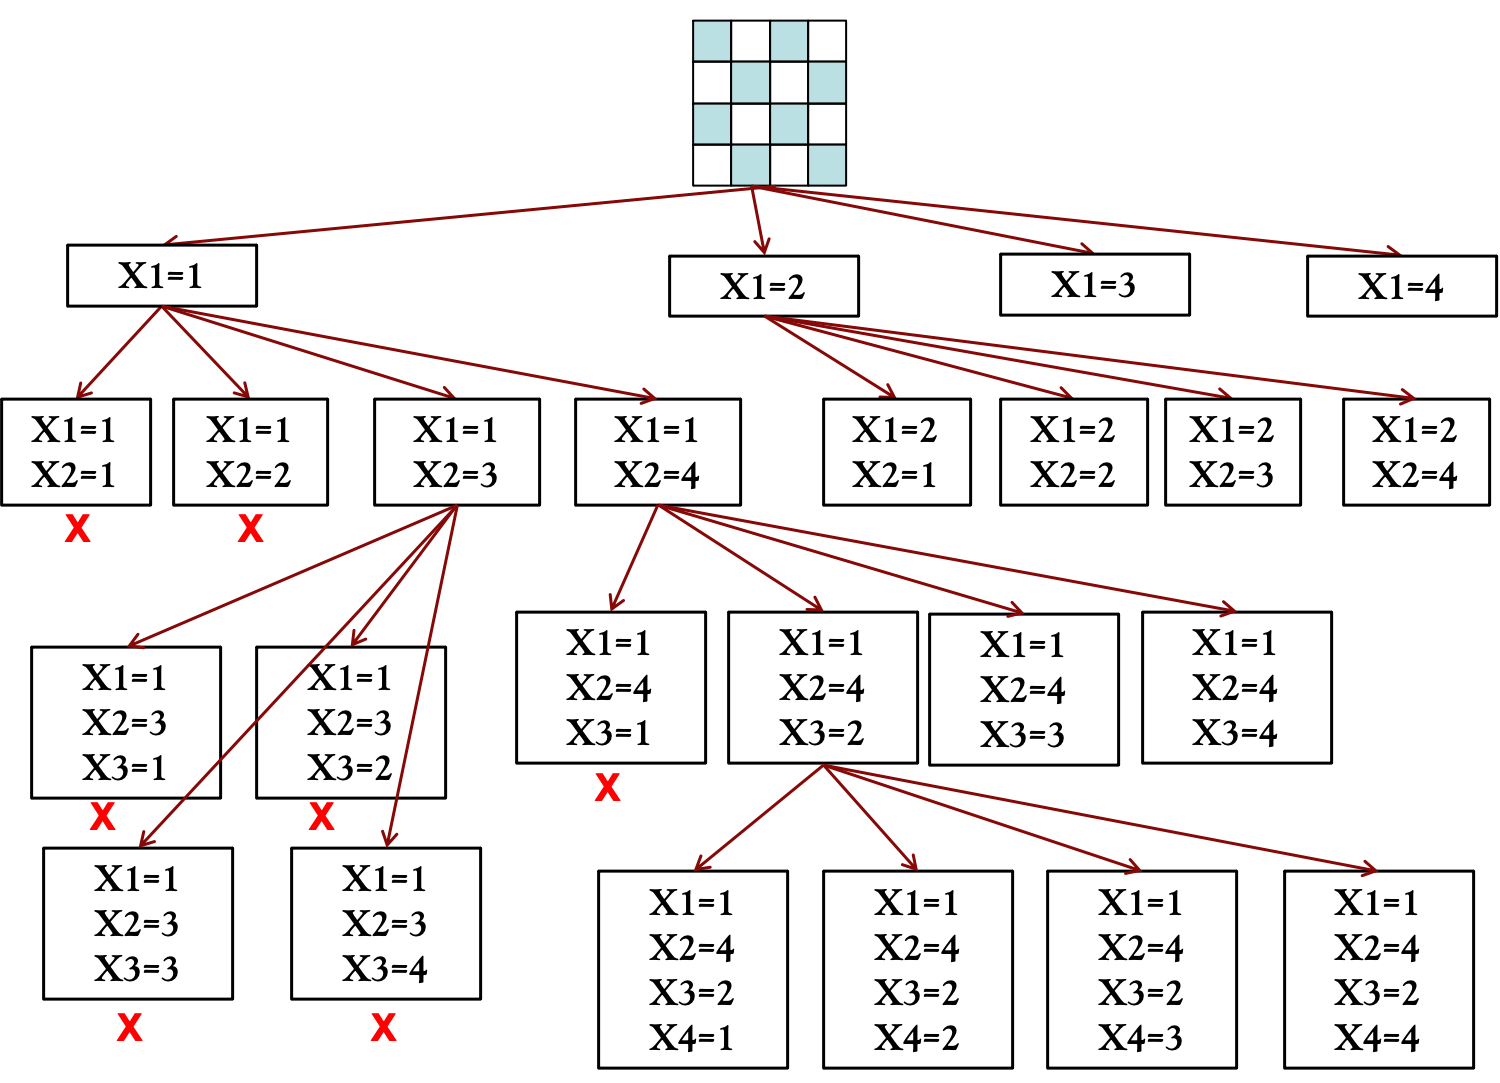
\includegraphics[scale=0.35]{./img/Back_NReinas}
\end{figure}

\end{frame} 

%%%%%%%%%%%%%%%%%%%%%%%%%%%%%%%%
\begin{frame}  \frametitle{Backtracking y Forward checking N Reinas} \footnotesize


\begin{figure}
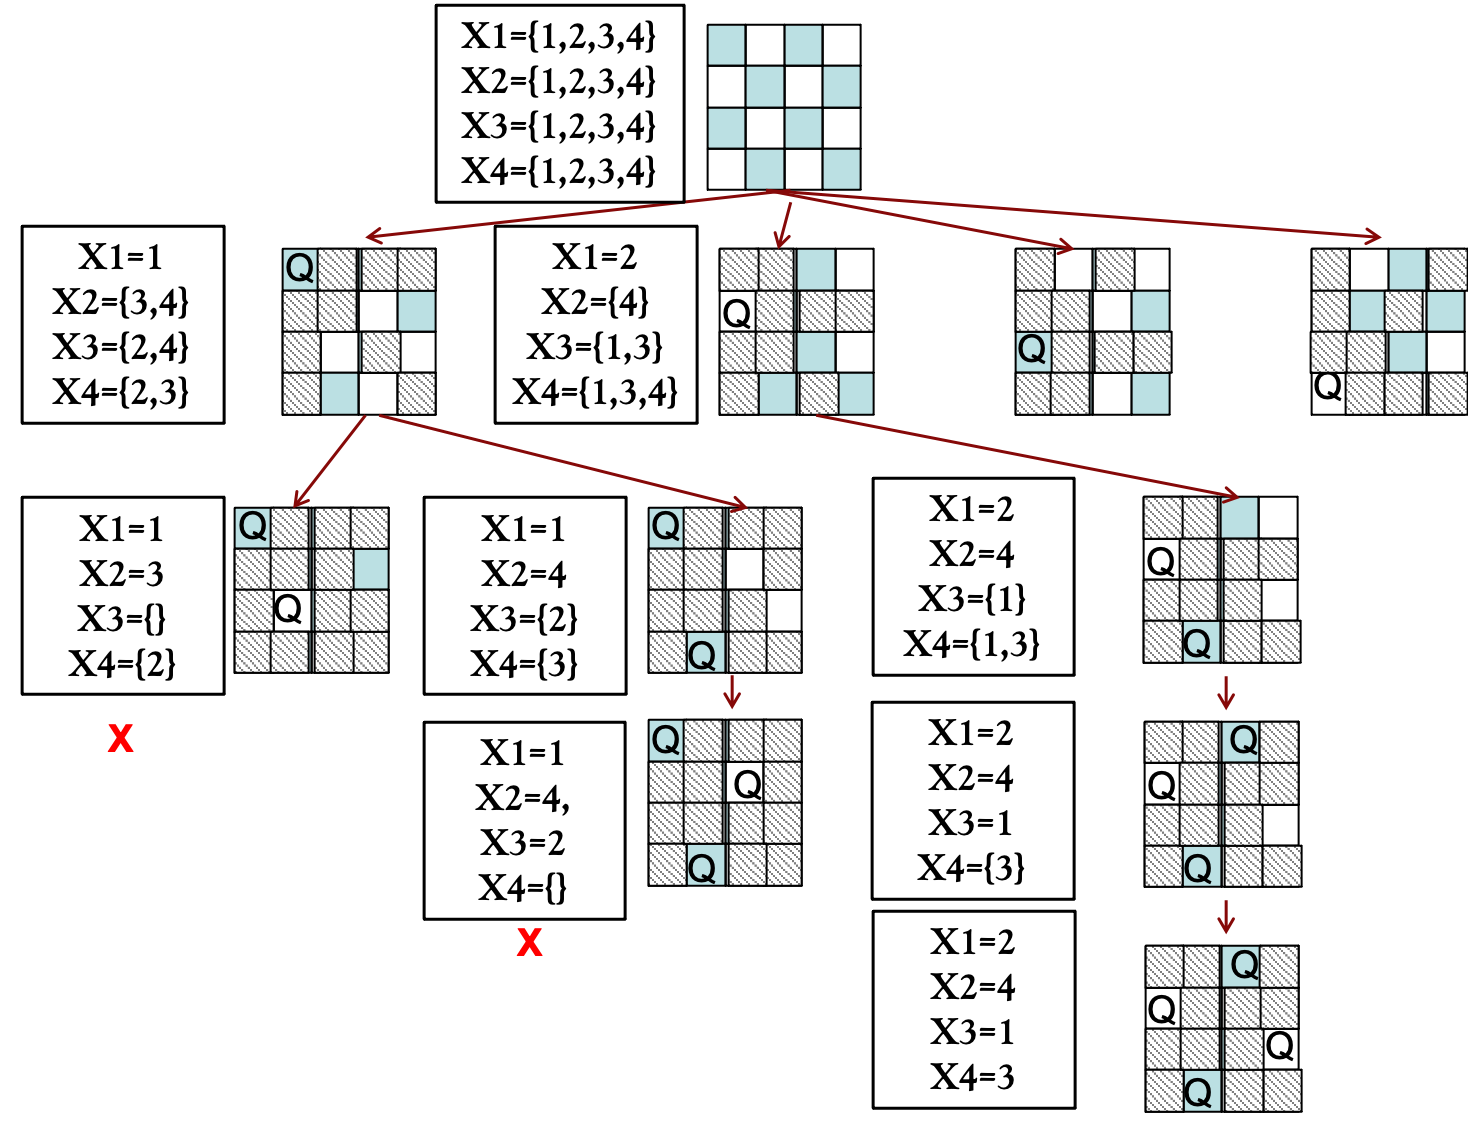
\includegraphics[scale=0.35]{./img/BC_FC_Nreinas}
\end{figure}

\end{frame} 

\subsection{Búsqueda Local}
%%%%%%%%%%%%%%%%%%%%%%%%%%%%%%%%
%%%%%%%%%%%%%%%%%%%%%%%%%%%%%%%%


%%%%%%%%%%%%%%%%%%%%%%%%%%%%%%%%
\begin{frame}  \frametitle{Búsqueda Local} \small

\begin{itemize}
\item  Los algoritmos de búsqueda local pueden ser efectivos para resolver algunos problemas de CSP.
\item El estado inicial establece un valor a cada variable
\item  Y la búsqueda cambia el valor de una variable cada paso.
\item  La solución inicial normalmente no cumplirá las restricciones, el objetivo es que se cumplan las restricciones. 

\end{itemize}

\end{frame} 

%%%%%%%%%%%%%%%%%%%%%%%%%%%%%%%%
\begin{frame}  \frametitle{Búsqueda Local} \small

\begin{itemize}
\item  Para escoger variable, la mejor heurística es seleccionar aquella que tiene un menor número de conflictos con otras variables (Min-conflicts heurístic)

\end{itemize}

\begin{figure}
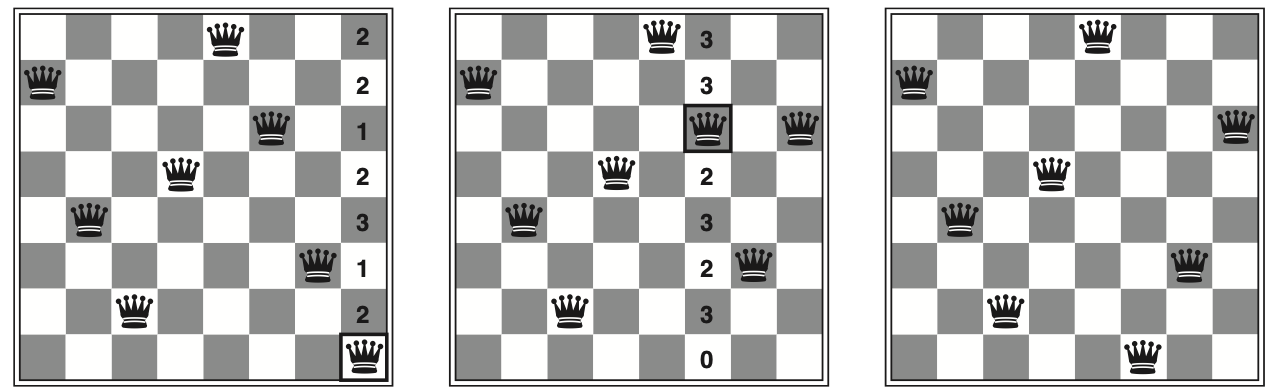
\includegraphics[scale=0.35]{./img/BLTablero}
\end{figure}

\end{frame} 
%%%%%%%%%%%%%%%%%%%%%%%%%%%%%%%%
\begin{frame}  \frametitle{Búsqueda Local} \small


\begin{figure}

\includegraphics[scale=0.5]{./img/BLImagen}
\end{figure}

\end{frame} 

%%%%%%%%%%%%%%%%%%%%%%%%%%%%%%%%
%%%%%%%%%%%%%%%%%%%%%%%%%%%%%%%%

\section{Resumen}
%%%%%%%%%%%%%%%%%%%%%%%%%%%%%%%%
%%%%%%%%%%%%%%%%%%%%%%%%%%%%%%%%

%%%%%%%%%%%%%%%%%%%%%%%%%%%%%%%%
\begin{frame}  \frametitle{Resumen} \scriptsize

Objetivo obtener las asignaciones de los valores de los dominios a las variables que cumplan las restricciones. 


\begin{enumerate}
\item  Identificar \\
Variables 			$V_1, V_2, V_3$\\
Dominios 		$D_1, D_2, D_3$\\
Restricciones	p.ej.  $V_1 \neq V_2$\\

\item  Intentar reducir los dominios. Aplicar las restricciones a los dominios originales.
\begin{enumerate} \scriptsize
\item Eliminación valores dominios.
\item  Aplicación algoritmo AC-3. 
\end{enumerate}

\item  Los dominios se han quedado vacío.  \textbf{No tengo solución } 
\item  Si los dominios son pequeños y dominios no vacíos.  \textbf{Solución problema}

\item Los dominios aún reduciendo son muy grandes pasamos a Backtracking para buscar solución al problema. 
\begin{enumerate} \scriptsize
\item 	Establecer un orden de las variables.
\item 	Establecer un orden de los dominios.
\item 	 Realizar inferencias, reducir los dominios una vez que tenga asignación
\end{enumerate}

\end{enumerate}



\end{frame} 
%\begin{frame} [fragile] \frametitle{Programación ``Tradicional''} \footnotesize
%
%\begin{minted}[frame=lines,framesep=2mm,baselinestretch=1.2,bgcolor=white,fontsize=\scriptsize,linenos]{java}
%
%\end{minted}
%
%\end{frame} 

%%%%%%%%%%%%%%%%%%%%%%%%%%%%%%%%
%%%%%%%%%%%%%%%%%%%%%%%%%%%%%%%%



 


%%%%%%%%%%%%%%%%%%%%%%%%%%%%%%%%
%\begin{frame}  \small  
%\end{frame} 


%%%%%%%%%%%%%%%%%%%%%%%%%%%%%%%%
%\begin{frame}  \small  
%\end{frame} 


%%%%%%%%%%%%%%%%%%%%%%%%%%%%%%%%
%\begin{frame}  \small  
%\end{frame} 


%%%%%%%%%%%%%%%%%%%%%%%%%%%%%%%%
%\begin{frame}  \small  
%\end{frame} 

%%%%%%%%%%%%%%%%%%%%%%%%%%%%%%%%
%%%%%%%%%%%%%%%%%%%%%%%%%%%%%%%%
\section{}

\begin{frame} %\frametitle{Preguntas}

%\begin{center}
%¡Gracias por su atención!\\
%\end{center}
\vspace*{2cm}

\begin{center}
\textbf{José A. Montenegro Montes} \\

\textit{Dpto. Lenguajes y Ciencias de la Computación}\\
\textit{ETSI  Informática. Universidad de Málaga}\\
\textbf{jmmontes@uma.es}
\end{center}

\vspace*{1,3cm}

 \hspace*{1.cm}
\includegraphics[height=0.1\textheight]{./img/logos/logoUma.png} \hspace*{2.5cm}

\includegraphics[height=0.1\textheight]{./img/logos/logoInf.png}   \hspace*{2.5cm}

\includegraphics[height=0.1\textheight]{./img/logos/logoLcc.png}  


\end{frame} 

\end{document} 
